%!TEX TS-program = xelatex
%!TEX encoding = UTF-8 Unicode

\documentclass[galley]{jtlu-article-2col} 
\usepackage{tabu}
\renewcommand\query[1]{\relax}

%\graphicspath{{../Graphics/},{../../../../jtlugraphics/}}

%% ===== BEGIN ARTICLE DATA BLOCK - FILL IN THIS STUFF ==== %%
%% ===== JTLU publication and copyright info (required) === %%
\jtluissue{0}
\jtluvolume{0}								    	   
\jtluyear{2021}								   
\jtlurights{Juste Raimbault}	 
\jtluid{nnn}
\setcounter{page}{1} 


\usepackage{bbm}
\usepackage{mdframed}


%% ===== ARTICLE TITLE (required), subtitle (optional) ==== %%
\title{Mapping the research landscape on modeling interactions between networks and territories}
%\subtitle{Subtitle in sentence case}

%% ===== SHORT TITLE (required for page headers) ========== %%
\shorttitle{Mapping the research landscape}

%% ===== AUTHOR INFORMATION (required) ==================== %%             
%% Name, affiliation/institution, and email/contact for each
%% Add as many as necessary, separated by "\and":

%\author{{\semibfsf Juste Raimbault  } \\UPS CNRS 3611 ISC-PIF and UMR CNRS 8504 G{\'e}ographie-cit{\'e}s  \thanks{Dr. juste.raimbault@polytechnique.edu}
\author{ Juste Raimbault  \\UPS CNRS 3611 ISC-PIF and UMR CNRS 8504 G{\'e}ographie-cit{\'e}s  \thanks{juste.raimbault@polytechnique.edu}
  % \and {\bfseries } \\ 
  % \and {\bfseries } \\    
}% End authors

%% ===== END ARTICLE DATA BLOCK =========================== %%

\date{} % SET DATE TO NOTHING; NO DATE ON PAPERS

\hypersetup{%
			pdftitle={Title},
			pdfauthor={Firstname Lastname},
			pdfproducer={The Journal of Transport and Land Use vol. 0 no. 0 }
			pdfstartpage=1,
			colorlinks=true,
			linkcolor=NavyBlue,
			citecolor=PineGreen,
			urlcolor=BrickRed			
} % END HYPERSETUP


\begin{document}
%\twocolumn[
%\begin{@twocolumnfalse}
\maketitle
\begin{abstract}
Research on transport and land-use is by essence interdisciplinary, as a result of the multiple dimensions of these objects yielding as much corresponding viewpoints. In the case of models dealing with interactions between transport and land-use, the research landscape is similarly rather disparate. We propose to contribute to research in this field by proposing maps of the research landscape.
\end{abstract}

\begin{keywords}
  Land-use Transport Interaction Modeling; Quantitative Epistemology; 
\end{keywords}
%\end{@twocolumnfalse}
%]
%\saythanks



%%%%%%%%%%%%%%%
\section{Introduction}
%%%%%%%%%%%%%%%

% context

We gave a broad overview of different types of models taking into account interactions between networks and territories, with disciplines and problematics that are associated. These very different aspects suggest a strong compartmentalization of disciplines. It is furthermore difficult to distinguish potential models of co-evolution within this fuzzy environment. We may legitimately ask what are the existing and potential relations between the different approaches? Which fields may have been missed although they are complementary?

Diverse hypotheses can be proposed in order to explain the absence of investigations on co-evolution models:
\begin{itemize}
	\item Following~\cite{commenges:tel-00923682}, scientific and operational actors that would be concerned by the practical application of such models would see themselves replaced by the same models and have thus no incentive to develop them (sociological explanation).
	\item The different disciplines which possess the diverse components that are necessary to such models are compartmentalized and have divergent motivations (epistemological explanation).
	\item The construction of such models exhibits intrinsic difficulties making their development not encouraging and not well currently tackled.
\end{itemize}

We will not be able in this work to explore the first assumption (or more precisely, it would require a subject in itself, implying in particular sociological interviews). The third is either a tautology or can not be demonstrated, in a Church style as it can be put, and our whole work will allow us to bring elements of answer. The second is on the contrary as we will see more within our reach.

A way to explore this hypothesis and to answer to previous questions relies in an epistemological study that we propose to lead in a quantitative and systematic way. This approach is complementary to the previous literature review, and allows both to contextualize it and to systematize it. We must also recall the idea that the study of reasons for a sparsity of models will necessarily inform on models themselves and on the questions relates to their construction: the \emph{knowledge of knowledge}~\cite{morin1986methode} increases the knowledge.


The empirical and thematic literature, together with the case studies previously developed, seem to converge towards a consensus on the complexity of relations between transportation networks and territories. In some configurations and at some scales, it is possible to exhibit circular causal relationships between territorial dynamics and transportation networks dynamics. We designate their existence through the concept of \emph{co-evolution}. It seems to be difficult to introduce simple or systematic explanations for these dynamics, as recall for example the debates around structuring effects of infrastructures~\cite{offner1993effets}.

Furthermore, the multiple geographical situations suggest a strong dependency to the context, giving a relevance to fieldwork and to targeted studies. But geographical explanation and the understanding of processes remains quickly limited in this approach, and intervenes a need for a certain level of generality. Its on such a point that the evolutive urban theory is focused in particular, since it allows to combine schemes and general models to the geographical particularities. On the contrary, some theories coming from physics applying to the study of urban systems~\cite{west2017scale} can be more difficult to accept for geographers because of their universality positioning which is on the opposite of their ordinary epistemologies.

In any case, the \emph{medium} which allows to gain in generality on processes and structures of systems is always the model. As J.P. Marchand puts it\footnote{Personal communication, May 2017.}, ``\textit{our generation has understood that there was a co-evolution, yours aims at understanding it}'', what insists on the power of understanding brought by modeling and simulation that we judge to be today still with a very high potential for development.



Without developing for now the numerous functions that a model can have, we will rely on the positioning of Banos which states that ``modeling is learning'', and following our positioning within a complex systems science suggested in introduction, we will thus make \emph{modeling interactions between networks and territories} our principal subject of study, tool, object\footnote{Even if after a rereading of this positioning at the light of~\ref{sec:knowledgeframework}, it has no meaning since our appproach already contained models as soon as it was scientific.}. This chapter must be taken as a ``state-of-the-art'' of approaches modeling interactions between networks and territories. It aims in particular at capturing different dimensions of knowledge: therefore, we will uses quantitative epistemology analyses.




In a first section~\ref{sec:modelingsa}, we review from an interdisciplinary perspective the models that can be linked, even remotely, without a priori of temporal or spatial scale, of ontologies, of structure, or of application context. This overview is possible thanks to the diverse disciplinary entries revealed in the previous chapter: for example geography, transportation geography, planning. This overview suggests relatively independent knowledge structures and disciplines that rarely communicate.


We proceed in~\ref{sec:quantepistemo} to an algorithmic systematic review, which corresponds to a reconstruction by iterative exploration of a scientific landscape. Its results tend to confirm this compartmentalization. The study is completed by a multilayer network analysis, combining citation network and semantic network obtained through text-mining, which allows to better grasp the relations between disciplines, their lexical field and their interdisciplinarity patterns.






%%%%%%%%%%%
\section{Literature review}

% "hand" overview


We develop now an overview of different approaches modeling interactions between networks and territories. First of all, we need to notice a high contingency of scientific constructions underlying these. Indeed, according to~\cite{bretagnolle2002time}, the ``\textit{ideas of specialists in planning aimed to give definitions of city systems, since 1830, are closely linked to the historical transformations of communication networks}''. The historical context (and consequently the socio-economical and technological contexts) conditions strongly the formulated theories. It implies that ontologies and corresponding models addressed by geographers and planners are closely linked to their current historical preoccupations, thus necessarily limited in scope and/or operationnal purpose. In a perspectivist vision of science~\cite{giere2010scientific}, such boundaries are the essence of the scientific entreprise, and as we will argue in chapter~\ref{ch:theory} their combination and coupling in the case of models is generally a source of knowledge.

The entry we take here to sketch an overview of models is complementary to the one taken in chapter~\ref{ch:thematic}, by declining them through their main object (i.e. the relations Network $\rightarrow$ Territory, Territory $\rightarrow$ Network and Territory $\leftrightarrow$ Network)\footnote{We recall the meaning of this notation introduced in chapter~\ref{ch:thematic}: a cirect arrow correspond to processes that we can relatively univocally attribute to the origin, whereas a reciprocal arrow assumes the intrinsic existence of reciprocal interaction, generally in coincidence with the emergence of entities playing a role in these.}.

The reference frame for scales is also the one introduced in~\cite{raimbault2018caracterisation}, knowing that we do not consider the microscopic scales with the choice of discarding daily mobility models. We have therefore roughly mesoscopic and macroscopic temporal and spatial scales.

We have seen that the correspondence to temporal and spatial scales is not systematic (see the provisional double entry typology for processes). On the contrary, the correspondence to fields of study and types of stakeholders is more systematic. This literature review is thus done following the latest logic.

One important approach to the modeling of the influence of transportation networks on territories lies in the field of planning, at medium temporal and spatial scales (the scales of metropolitan accessibility we developed before). Models in geography at other scales, such as the Simpop models already described~\cite{pumain2012multi}, do not include a particular ontology for transportation networks, and even if they include networks between cities as carriers of exchanges, they do not allow to study in particular the relations between networks and territories. We will come back later on extensions that are relevant for our question. First, let recall the context of models closer to planning studies.

\paragraph{LUTI models}

These approaches are generally named as \emph{models of the interaction between land-use and transportation} (\emph{LUTI}, for \textit{Land-Use Transport Interaction}). Land-use generally means the spatial distribution of territorial activities, generally classified into more or less precise typologies (for example housing, industry, tertiary, natural space). These works can be difficult to apprehend as they relate to different scientific disciplines\footnote{We make here the choice to gather numerous approaches having the common characteristic to principally model the evolution of land-use, on medium temporal and spatial scales. The unity and the relative positioning of these approaches covering from economics to planning, remain an open question that to the best of our knowledge has never been frontally tackled. The work done in~\ref{sec:quantepistemo} introduces elements of answer through an approach in quantitative epistemology.}. Their general principle is to model and simulate the evolution of the spatial distribution of activities, taking transportation networks as a context and significant drivers of localizations. To understand the underlying conceptual frame to most approaches, the Frame~\ref{frame:modelingsa:wegener} sums up the one given by \cite{wegener2004land}\footnote{A more general frame that we already developed, that allows to bridge it with our frame, is the one given by~\cite{le2010approche}, which situates the triad Transportation system/Localization system/Activities system within the relation with agents: agents creating demand, agents building the city, external factors.}.

For example, from the point of view of urban economics, propositions for such models have existed for a relatively long time: \cite{putman1975urban} recalls the frame of urban economics in which main components are employments, demography and transportation, and reviews economic models of localization that relate to the Lowry model already mentioned.





%%%%%%%%%%%%%%
\begin{figure}[h!]
	\begin{mdframed}
		
		\cite{wegener2004land} introduces a general theoretical and empirical frame for land-use transport interaction models. The four concepts included are land-use, localization of activities, the transportation system and the distribution of accessibility. A cycle of circular effects are summed up in the following loop:
		
		\begin{center}
		\bigskip
	
		%\tikzmark{Activities} $\longrightarrow$ Transportation system $\longrightarrow$ Accessibility $\longrightarrow$ Land-\tikzmark{use}\arrow{use}{Activities}
				
		\bigskip
		\end{center}
		
		The transportation system is assumed with a \emph{fixed infrastructure}, i.e. effects of the distribution of activities are effects on the \emph{use} of the transportation system (and thus link to \emph{mobility} in our more general frame): modal choice, frequency of trips, length of travels.
	
		
		The theoretically expected effects are classified according to the direction of the relation (\textit{Land-use}$\rightarrow$\textit{Transport} or \textit{Transport}$\rightarrow$\textit{Land-use}, and a loop \textit{Transport}$\rightarrow$\textit{Transport} that is not taken into account in our case), and according to the acting factor (residential density, of employments, localization, accessibility, transportation costs) and also by the aspect that is modified (length and frequency of trips, modal choice, densities, localizations). We can for example take:
		\begin{itemize}
		\item \textit{Land-use}$\rightarrow$\textit{Transport}: a minimal residential density is necessary for the efficiency of public transportation, a concentration of employments implies longer trips, larger cities have a greater proportion of the modal part of public transportation.
		\item \textit{Transport}$\rightarrow$\textit{Land-use}: a high accessibility implies higher prices and an increased development of residential housing, companies locate for a better accessibility to transportation at a larger scale.
		\item \textit{Transport}$\rightarrow$ \textit{Transport}: places with a good accessibility will produce more and longer trips, modal choice and transportation cost are highly correlated. 
		\end{itemize}
				
		These theoretical effects are then compared to empirical observations, which for most of them give the way processes are implemented. Some are not observed in practice, whereas most converge with theoretical expectations.		
			
		
		\bigskip
		
		\textit{Comment 1: An uniscalar framework ?} This framework takes schematically into account two main scales, the scale of daily mobility and the scale of the localization of activities. Knowing that in practice mobility behaviors are generally taken into account as average flows, it often reduces to a unique mesoscopic scale. All in all, it does not allow to take into account dynamics on longer time scales, that would include the evolution of the transportation network infrastructure or structural dynamics of systems of cities on long time periods.
				
		
		\bigskip
		
		\textit{Comment 2: A systematic view of structuring effects ?} Furthermore, critics of the rhetoric of structuring effects may find in this framework its strong presence, since direct effects of accessibility on land-use and then the localization of activities are assumed here. These critics can be undermined by observing that these are theoretical expected effects, and that the framework is put into perspective of empirical effects indeed observed. We will however always take it with caution, by situating it in terms of context and scales.
				
		\bigskip
		
		\textbf{Conceptual framework of land-use transport interactions according to \cite{wegener2004land}.}\label{frame:modelingsa:wegener}
	\end{mdframed}
\end{figure}
%%%%%%%%%%%%%%




\cite{wegener2004land} give more recently a state of the art of empirical studies and in modeling on this type of approach of interactions between land-use and transport. The theoretical positioning is closer of disciplines such as transportation socio-economics and planning (see the disciplinary landscapes described in~\ref{sec:quantepistemo}). \cite{wegener2004land} compare and classify seventeen models, among which no one includes an endogenous evolution of the transportation network on relatively short time scales for simulations (of the order of the decade). We find again indeed the correspondance with typically mesoscopic scales previously established. A complementary review is done by~\cite{chang2006models}, broadening the context with the inclusion of more general classes of models, such as spatial interactions models (which contain trafic assignment and four steps models), planing models based on operational research (optimization of locations of different activities, generally homes and employments), the microscopic models of random utility, and models of the real estate market.


%%%%%%%%%%%%%%
\begin{figure}
	\begin{mdframed}

	The Pirandello\textregistered model\footnote{The origin of the name is not given, but strongly suggests the influence of its original creators V. Piron and J. Delons.} is presented in \cite{delons:hal-00319087} as one of the first attempts to develop an operational Luti model in France. The model is based on four fundamental economic processes: the real estate market and the dwellings offer, the residential mobility of households, the attribution of travel destinations, the model choice. The model is static, i.e. computes n equilibrium for spatial distributions of actives and employments, and also for transportation flows.
		
	
	The fundamental processes taken into account and their implementation are the following:
	\begin{itemize}
		\item Residential choices of households are based on a utility function taking into account (i) a confort term as a Cobb-Douglas of housing surface and income, corrected by a linear preference for individual dwellings; (ii) an accessibility term based on generalized cost (aggregation of transportation cost and time, with a value of time); (iii) the dwelling price and the local tax as a function of the housing surface; (iv) a fixed effect by income and by area; and (v) a random term assumed to follow a Gumbel law. Location probabilities for an income group are then given by a discrete choice model given this utility.
		\item The housing prices are formed following a scaling law of population.
		\item A local bidding mechanism answers to the demand previously obtained, as a function of an exogenous dwelling offer.
		\item Companies locate by maximizing their profit, function of the productivity (Cobb-Douglas in the salary and the accessibility) and the real estate price, under the constraint of a fixed spatial distribution of the number of employments, of the office surface, and of the total production of the region.
		\item Transportation is taken into account through a four steps model, which distributes model choices and destination choices with a discrete choice model, and flows are assigned according to a Wardrop equilibrium (see~\ref{sec:reproducibility}), what allows to adjust the values of accessibility given a spatial distribution of activities.
	\end{itemize}
		
	
	The mechanism to combine these different processes to obtain a global equilibrium is detailed by~\cite{kryvobokov2013comparison}, and consists in the establishment of three sub-equilibriums at different scales: transportation flows (giving costs) on a short term, location and real estate prices on the middle term, land prices and available terrains (fixed in an exogenous way for all the modeled period).
	
	\bigskip
	
	
	\textit{Commentary: Equilibrium, operational model and calibration.} A certain number of remarks can be done concerning this model, the most important for our approach are: (i) the equilibrium assumption can be a powerful tool to understand the structure of the attractors of the system, but has no empirical foundation, and even less for the coupling of equilibriums at different scales; (ii) thus, the operational nature of the model can be discussed, since the study of the impact of scenarios on the movements of attractors can difficultly allow to infer on local dynamics of the system; and (iii) sub-models are calibrated more or less rigorously and relatively separately, but the conditions of a calibration by decomposition are an open question still not well explored and linked to the nature of model coupling. In our sense, such a micro-based model would in any case be in better consistence with a philosophy of dynamical generative modeling and parsimony (see\ref{sec:computation}).
	
	\medskip
	
	\textbf{The Pirandello model.}\label{frame:modelingsa:pirandello}
	
	\end{mdframed}
\end{figure}
%%%%%%%%%%%%%%	

	
	
	
	
%%%%%%%%%%%%%%
\begin{figure}
	\begin{mdframed}
	
	The Nedum2D model, described in details by~\cite{viguie2014downscaling}, is focused on the localization of actives and their interaction with land rent and real estate promoters: it is a model inspired by the Fujita-Ogawa model~\cite{fujita1982multiple}, inheriting from the literature in Urban Economics.
	
	The processes included in the model are, with each its own time scale fixed by a parameter:
	\begin{itemize}
		\item Households make a compromise between housing surface and available budget without transportation costs and rent, following a Cobb-Douglas function for the corresponding utility. This process induces a dynamic for housing surface as a function of the distance to the center.
		\item They relocate in order to have an expected utility larger than the average.
		\item Rents evolve to maximize the occupation or in response to an external demand.
		\item New buildings are built by promoters that aim at maximizing their profits.
	\end{itemize}
	
	
	This model is dynamical and simulates the evolution of these different variables in space (the formulation above is monocentric, a polycentric extension and one taking into account an exogenous distribution of employments exist) and time. Its spatial scale is metropolitan, and the time scale can range from a medium scale (decade) to longer time-periods (century), knowing that the latest has a low credibility since it keeps static numerous other components of the urban system.
	
		
	\medskip
	
	
	\textit{Comment: extension of ontologies.} The coupling of Nedum with a model for traffic assignment, the Modus model\footnote{In the frame of the current research project ANR VITE! (see \url{http://www.agence-nationale-recherche.fr/Projet-ANR-14-CE22-0013}).}, aims at including the feedback of congestion in the transportation system on costs, and thus on the localization and on the urban structure. Fundamental questions arise from the first coupling experiments:
	\begin{itemize}
		\item Is the masterplan \emph{Schéma Directeur} really useful, since is seems to only accompany already existing dynamics ? In other words, \textit{is the governance process endogenous} ? Does the Sdrif in fact capture an intrinsic dynamic on a longer time ?
		\item The coupling of models raises in itself technical difficulties, for communication between modules already implemented in different languages and for convergence of the coupled model in a reasonable number of iterations.
		\item It furthermore raises ontological difficulties: each model includes opposite mechanisms for the same ontology (aggregation effect against congestion effect for the distribution of population). The question is then if a specific coupling ontology is necessary (for example with specific equations integrating these contradictory effects), to allow on the one hand a better convergence, on the other hand a better ontological consistency.
	\end{itemize}
	
		
	
	% couplage avec modus http://www.agence-nationale-recherche.fr/Projet-ANR-14-CE22-0013
	% seminaire lvmt (27/11) : points cruciaux soulevés
	%  - endogeneite de la gouvernance, ou le sdrif sert-il a rien ? accompagne dynamique locale. negociations locales. modele calibre sur amenagements passes : le sdrif n'est pas une rupture : dynamique sur le temps long intrinseque, capturee par le modele.
	%  - difficulte technique du couplage : ouverture etc
	%  - question endogeneite : White, exploration modeles, mutlimodeling, parcimonie.
	%  - difficulte ontologique du couplage : modele ont processus oppose, instable numeriquement : domaines de validités locaux ? (au sens des hypotheses) - en ouverture : enrome a travail a faire sur le couplage, du point de vue des domaines de connaissance (differentes dimensions du couplage)
	
	\medskip
	
	\textbf{The Nedum model.}\label{frame:modelingsa:nedum}	
	\end{mdframed}
\end{figure}
%%%%%%%%%%%%%%




In order to give a better intuition of the logic underlying some Luti models, we detail in Frame~\ref{frame:modelingsa:pirandello} and in Frame~\ref{frame:modelingsa:nedum} the structures, the ontologies, and assumptions of two models developed in the specific case of Ile-de-France (allowing on the one hand a comparison between both and on the other hand echoing the thematic development of~\ref{sec:casestudies}). Even for very close ontologies (real estate prices, households localizations), we see the variety of possible assumptions and of issues raised by the models.

\paragraph{Very different operational models}

The variety of existing models lead to operational comparisons: \cite{paulley1991overview} synthesize a project comparing different model applied to different cities. Their result allow on the one hand to classify interventions depending on their impact on the level of interaction between transportation and land-use, and on the other hand to show that the effects of interventions strongly depend on the size of the city and on its socio-economic characteristics.

Ontologies of processes, and more particularly on the question of equilibrium, are also varied. The respective advantages of a static approach (computation of a static equilibrium of households localisation for a given specification of their utility functions) and of a dynamical approach (out-of-equilibrium simulation of residential dynamics) has been studied by~\cite{kryvobokov2013comparison}, within a metropolitan frame on time scales of the order of the decade. The authors show that results are roughly comparable and that each model has its utility depending on the question asked.

Different aspects of the same system can be included within diverse models, as show for example~\cite{wegener1991one}, and traffic, residential and employments dynamics, the evolution of land-use as a consequence, also influenced by a static transportation network, are generally taken into account. \cite{iacono2008models} covers a similar horizon with an additional development on cellular automata models for the evolution of land-use and agent-based models. The temporal range of application of these models, around the decade, and their operational nature, make them useful for planning, what is rather far of our focus to obtain explicative models of geographical processes. Indeed, it is often more relevant for a model used in planning to be understandable as an anticipation tool, or even a communication tool, than to be faithful to territorial processes, at the cost of an abstraction.

\paragraph{Perspectives for LUTI models}

\cite{timmermans2003saga} formulates doubts regarding the possibility of interaction models that would be really integrated, i.e. producing endogenous transportation patterns and being detached from artefacts such as accessibility for which the influence of its artificial nature remains to be established, in particular because of the lack of data and a difficulty to model governance and planning processes. It is interesting to note that current priorities for the development of LUTI models seem to be centered on a better integration of new technologies and a better integration with planning and decision-making processes, for example through visualization interfaces as proposed by~\cite{JTLU611}. They do not aim at being extended on problematics of territorial dynamics including the network on longer time scales for example, what confirms the range and the logic of use and development of this type of models.

A generalization of this type of approach at a smaller scale, such as the one proposed by \cite{russo2012unifying}, consists in the coupling between a LUTI at the mesoscopic scale to macroeconomic models at the macroscopic scale\footnote{\cite{russo2012unifying} indeed generalizes the framework of LUTI models to propose a framework of interaction between spatial economy and transportation (\emph{Spatial Economics and Transport Interactions}). This framework includes LUTI models at the urban scale, and at the national level macroeconomic models simulating production and consumption, competition between activities, production of the stock of the offer of transportation. Transportation models still assume a fixed network and establish equilibria within it, what implies a small spatial scale and a short time scale.}. These do not consider the evolution of the transportation network in an explicit manner but are interested only to abstract patterns of demand and offer. Urban economics have developed specific approaches that are similar in their context: \cite{masso2000} for example describes an integrated model coupling urban development, relocations and equilibrium of transportation flows.

Thus, we can synthesize this type of approach, that we can designate through a semantic shortcut as \emph{LUTI approaches}, by the fundamental following characteristics: (i) models aiming at understanding an evolution of the territory, within the context of a given transportation network; (ii) models in a logic of planning and applicability, being themselves often implied in decision-making; and (iii) models at medium scales, in space (metropolitan scale) and in time (decade).


\subsubsection{Network Growth}

We can now switch to the ``opposite'' paradigm, focused on the evolution of the network. It may seem strange to consider a variable network while neglecting the evolution of the territory, when considering the overview of some potential evolution mechanisms we previously reviewed (potential breakdown, self-reinforcements, network planning) which occur at mainly longer time scales than territorial evolutions. We will see here that there is no paradox, since (i) either the modeling focuses on the evolution of \emph{network properties}, at a short scale (micro) for congestion, capacity, tarification processes, mainly from an economic point of view; (ii) or territorial components playing indeed a role on the network are stable on the long scales considered.

Network growth is the subject of modeling approaches which aim at explaining the growth of transportation networks. They generally take a \emph{bottom-up} and endogenous point of view, i.e. aiming at unveiling local rules that would allow to reproduce the growth of the network on long time scales (often the road network). As we will see, it can be a topological growth (creation of new links) or the growth of link capacities in relation with their use, depending on scales and ontologies considered. To simplify, we distinguish broad disciplinary streams having studied the modeling of the growth of transportation networks: these are respectively linked to transportation economics, physics, transportation geography, and biology.

We thus partly rejoin the classification by~\cite{xie2009modeling}, which proposes an extended review of modeling the growth of transportation networks, in a perspective of transportation economics but broadened to other fields. \cite{xie2009modeling} distinguishes broad disciplinary streams having studied the growth of transportation networks: transportation geography has developed very early models based on empirical facts but which have focused on reproducing topology rather than mechanisms\footnote{According to \cite{xie2009modeling}, the contribution of geography consists in limited efforts at the period of \cite{haggett1970network}, we will therefore build on this review and not give a more thorough development.}; statistical models on case studies produce very limited conclusions on causal relations between network growth and demand (growth being in that case conditioned to demand data); economists have studied the production of infrastructure both from a microscopic and macroscopic point of view, generally not spatialized; network science has produced stylized models of network growth which are based on topological and structural rules rather than rules built on processes corresponding to empirical facts.

\paragraph{Economics}

Economists have proposed models of this type: \cite{zhang2007economics} reviews transportation economics literature on network growth, recalling the three main features studied by economists on that subject, that are road pricing, infrastructure investment and ownership regime, and finally describes an analytical model combining the three. These three classes of processes are related to an interaction between microscopic economic agents (users of the network) and governance agents. Models can include a detailed description of planning processes, such as~\cite{levinson2012forecasting} which combines qualitative surveys with statistics to parametrize a network growth model.  \cite{xie2009jurisdictional} compares the relative influence of centralized (planning by a governance structure) and decentralized growth processes (local growth which does not enters the frame of a global planning). 
 \cite{yerra2005emergence} shows through a reinforcement economic model including investment rule based on traffic assignment that local rules are enough to make hierarchy of roads emerge for a fixed land-use. \cite{levinson2003induced} proceed to an empirical study of drivers of road network growth for \emph{Twin Cities} in the United States (Minneapolis-Saint-Paul), establishing that basic variables (length, accessibility change) have the expected behavior, and that there exists a difference between the levels of investment, implying that local growth is not affected by costs, what could correspond to an equity of territories in terms of accessibility. The same data are used by~\cite{zhang2016model} to calibrate a network growth model which superimposes investment decisions with network use patterns. \cite{yerra2005emergence} shows with an economic model based on self-reinforcement processes (i.e. that include a positive feedback of flows on capacity) and which includes an investment rule based on traffic assignment, that local rules are sufficient to make a hierarchy of the road network emerge with a fixed land-use. A synthesis of these works gravitating around \noun{Levinson} is done in~\cite{xie2011evolving}.
 
 \paragraph{Physics}
 
 Physics has recently introduced infrastructure network growth models, largely inspired by this economic literature: a model which is very similar to the last we described is given by~\cite{louf2013emergence} with simpler cost-benefit functions by obtaining a similar conclusion. Given a distribution of nodes (cities)\footnote{We are here in a case in which the assumption of non-evolving city populations whereas the networks is iteratively established finds little empirical or thematic support, since we showed that network and cities had comparable evolution time scales. This models is thus closer to produce in the proper sense a \emph{potential network} given a distribution of cities, and must be interpreted with caution.} which population follows a power law, two cities will be connected by a road link if a cost-benefit utility function, which linearly combines potential gravity flow and construction cost\footnote{What gives a cost function of the form $C = \beta / d_{ij}^{\alpha} - d_{ij}$, where $\alpha$ and $\beta$ are parameters.}, has a positive value. These simple local assumptions are sufficient to make a complex network emerge with phase transitions as a function of the relative weight parameter in the cost function, leading to the emergence of hierarchy. \cite{zhao2016population} apply this model in an iterative way to connect intra-urban areas, and shows that taking into account populations in the cost function significantly changes the topologies obtained.
 
 An other class of models, close to procedural models in their ideas, are based on local geometric optimization processes, and aim at resembling real networks in their topology. \cite{bottinelli2017balancing} thus study a tree growth model applied to ant tracks, in which maintenance cost and construction cost both influence the choice of new links. The morphogenesis model by~\cite{courtat2011mathematics} which uses a compromise between realization of interaction potentials and construction cost, and also connectivity rules, reproduces in a stylized way real patterns of street networks. A very close model is described in~\cite{rui2013exploring}, but including supplementary rules for local optimization (taking into account degree for the connection of new links). Optimal network design, belonging more to the field of engineering, uses similar paradigms: \cite{vitins2010patterns} explore the influence of different rules of a shape grammar (in particular connection patterns between links of different hierarchical levels) on performances of networks generated by a genetic algorithm.


We can detail the mechanisms of one of these geometrical growth models. \cite{barthelemy2008modeling} describe a model based on a local optimization of energy which generates road networks with a globally reasonable shape. The model assumes ``centers'', which correspond to nodes of a road network, and road segments in space linking these centers. The model starts with initial connected centers, and proceeds by iterations to simulate network growth the following way:
\begin{enumerate}
	\item New centers are randomly added following an exogenous probability distribution, at fixed duration time steps.
	\item The network grows following a cost minimization rule: centers are grouped by projection on the network; each group makes a fixed length segment grow in the average direction towards the group starting from the projection (except if it vanishes in length, a segment then grows in the direction of each point).
\end{enumerate}
This model is adjusted in order that areas of parcels delimited by the network follow a power law with an exponent similar to the one observed for the city of Dresde. It has the advantage to be simple, to have few parameters (probability distribution for centers, length of segments built), to rely on reasonable local rules. This last point has also a dark side, since we can then expect the model to only capture few complexity, by neglecting numerous processes unveiled in chapter~\ref{ch:thematic} such as governance.



\paragraph{Biological networks}

Finally, an interesting and original approach to network growth are biological networks. This approach belongs to the field of morphogenetic engineering, which aims at conceiving artificial complex systems inspired from natural complex systems and on which a control of emerging properties is possible~\cite{doursat2012morphogenetic}. \emph{Physarum machines}, which are models of a self-organized mould (\emph{slime mould}) have been proved to solve in an efficient way difficult problems (in the sense of their computational complexity, see~\ref{sec:epistemology}) such as routing problems~\cite{tero2006physarum} or NP-complete navigation problems such as the Traveling Salesman Problem~\cite{zhu2013amoeba}. These properties allow these systems to produce networks with Pareto-efficient properties for cost and robustness~\cite{tero2010rules} which are typical of empirical properties of real networks, and furthermore relatively close to these in terms of shape (under certain conditions, see~\cite{adamatzky2010road}).

This type of models can have an interest in our case since self-reinforcement processes based on flows are analogous to link reinforcement mechanisms in transportation economics. This type of heuristic has been tested to generate the French railway network by~\cite{mimeur:tel-01451164}, making an interesting bridge with investment models by \noun{Levinson} we previously described\footnote{Knowing that for this study, validation criteria that were applied remain however limited, either at a level inappropriate to the stylized facts studied (number of intersection or of branches) or too general and that can be reproduced by any model (total length and percentage of population deserved), and belong to criteria of form that are typical to procedural modeling which can only difficultly account of internal dynamics of a system as previously developed. Furthermore, taking for an external validation the production of a hierarchical network reveals an incomplete exploration of the structure and the behavior of the model, since through its preferential attachment mechanisms it must mechanically produce a hierarchy. Thus, a particular caution will have to be given to the choice of validation criteria.}.


\paragraph{Procedural modeling}

Finally, we can mention other tentatives such as~\cite{de2007netlogo,yamins2003growing}, which are closer to procedural modeling~\cite{lechner2004procedural,watson2008procedural} and therefore have only little interest in our case since they can difficultly be used as explicative models\footnote{Following~\cite{varenne2017theories}, an explicative model allows to produce an explanation to observed regularities or laws, for example by suggesting processes which can be at their origin. If model processes are explicitly detached from a reasonable ontology, they can not be potential explanations. We will give in~\ref{sec:computation} a development of this notion in the frame of a more global reflexion on the epistemology of modeling.}. Procedural modeling consists in generating structures in a way similar to shape grammars\footnote{A shape grammar is a formal system (i.e a set of initial symbos, axioms, and a set of transformation rules) which acts on geometrical objects. Starting from initial patterns, they allow to generate classes of objects.}, but it also concentrates generally on the faithful reproduction of local form, without considering macroscopic emerging properties. Classifying them as morphogenesis models is incorrects and corresponds to a misunderstanding of mechanisms of \emph{Pattern Oriented Modeling}~\cite{grimm2005pattern}\footnote{\emph{Pattern Oriented Modeling} consists in seeking to explain observed patterns, generally at multiple scales, in a \emph{bottom-up} way. Procedural modeling does not correspond to that, since it aims at reproducing and not at explaining.} on the one hand and of the epistemology of morphogenesis on the other hand (see~\ref{sec:interdiscmorphogenesis}). We will use this type of models (exponential mixture to produce a population density for example) to generate initial synthetic data uniquely to parametrize other complex models (see~\ref{sec:computation} and \ref{sec:correlatedsyntheticdata}).

\subsection{Modeling co-evolution}

We can now switch to models that integrate dynamically the paradigm Territory $\leftrightarrow$ Network, which as we recall assumes that the conditioning of one by the other can not be identified. The ontologies used, as we will see, often couple\footnote{We recall the definition of model coupling, which corresponds to the one of system or process coupling given in introduction: it is the construction of a model that is simultaneously the extension of each initial model.} network elements with territorial components, but this positioning is not necessary and some elements may be hybrid (for example a governance structure for the transportation network may simultaneously belong to both aspects). In our reading of models, these different specifications will naturally arise.

We will broadly designate by model of co-evolution simulation models that include a coupling of urban growth dynamics and transportation network growth dynamics. These are relatively rare, and for most of them still at the stage of stylized models. The efforts being relatively sparse and in very different domains, there is not much unity in these approaches, beside the abstraction of the assumption of an interdependency between networks and territorial characteristics in time. We propose to review them still through the prism of scales.


\subsubsection{Microscopic and mesoscopic scales}


\paragraph{Geometrical Models}

\cite{achibet2014model} describes a co-evolution model at a very large scale (scale of the building), in which evolution of both network and buildings are ruled by a same agent, influenced differently by network topology and population density, and that can be understood as an agent of urban development. The model allows to simulate an auto-organized urban extension and to produce district configurations. Even if it strongly couples territorial components (buildings) and the road network, described results do not imply any conclusion on the processes of co-evolution themselves.

A generalization of the geometrical local optimization model described before is developed in~\cite{barthelemy2009co}. It aims at capturing the co-evolution of network topology with the density of its nodes. The localization of new nodes is simultaneously influenced by density and centrality, yielding the looping of the strong coupling. More precisely, the global behavior of the model is the same, as the network extension behavior. Centers then localize following a utility function that is a linear combination of average betweenness centrality in a neighborhood and of the opposite of density (dispersion due to higher price as a function of density). This utility is used to compute the probability of localization of new centers following a discrete choices model. The model allows to show that the influence of centrality reinforces aggregation phenomena (in particular through an analytical resolution on a one-dimensional version of the model), and furthermore reproduces exponentially decreasing density profiles (Clarcke's law) which are observed empirically. 

\cite{ding2017heuristic} introduce a model of co-evolution between different layers of the transportation network, and show the existence of an optimal coupling parameter in terms of inequalities for the centrality in network conception: if the road network is assimilated at a fine granularity to a population distribution, this model can be compared with the precedent model of co-evolution between the transportation network and the territory.

\paragraph{Economic models}

\cite{levinson2007co} take an economic approach, which is richer from the point of view of network development processes implied, similar to a four step model (i.e. including the generation of origin-destination flows and the assignment of traffic in the network) including travel cost and congestion, coupled with a road investment module simulating toll revenues for constructing agents, and a land-use evolution module updating actives and employments through discrete choice modeling. The exploration experiments show that co-evolving network and land uses lead to positive feedbacks reinforcing hierarchies. These are however far from satisfying, since network topology does not evolve as only capacities and flows change within the network, what implies that more complex mechanisms (such as the planning of new infrastructures) on longer time scales are not taken into account. \cite{li2016integrated} have recently extended this model by adding endogenous real estate prices and an optimization heuristic with a genetic algorithm for deciding agents.


From an other point of view, \cite{levinson2005paving} is also presented as a model of co-evolution, but corresponds more to a predictive model based on Markov chains, and thus closer to a statistical analysis than a simulation model based on these processes. \cite{rui2011urban} describe a model in which the coupling between land-use and network topology is done with a weak paradigm, land-use and accessibility having no feedback on network topology, the land-use model being conditioned to the growth of the autonomous network.



\paragraph{Cellular automatons}

A simple hybrid model explored and applied to a stylized planning example of the functionnal distribution of a new district in~\cite{raimbault2014hybrid}, relies on mechanisms of accessibility to urban activities for the growth of settlements with a network adapting to the urban shape. The rules for network growth are too simple to capture more elaborated processes than just a simple systematic connection (such as potential breakdown for example), but the model produces at a large scale a broad range of urban shapes reproducing typical patterns of human settlements. This model is inspired by~\cite{moreno2012automate} for its core mechanisms but yield a much broader generation of forms by taking into account urban functions.

At these relatively large scales, spanning from the urban to the metropolitan scale, mechanisms of population localization influenced by accessibility coupled to mechanisms of network growth optimizing some particular functions seem to be the rule for this kind of models: in the same way, \cite{wu2017city} couple a cellular automaton for population diffusion to a network optimizing local cost that depends on the geometry and on population distribution.

Models answering to more remote questions can furthermore be linked to our problem: for example, in a conceptual way, a certain form of strong coupling is also used in~\cite{bigotte2010integrated} which by an approach of operational research propose a network design algorithm to optimize the accessibility to amenities, taking into account both network hierarchy and the hierarchy of connected centers.


This way, co-evolution models at the microscopic and mesoscopic scales globally have the following structure: (i) processes of localization or relocalization of activities (actives, buildings) influenced by their own distribution and network characteristics; (ii) network evolution, that can be topological or not, answering to very diverse rules: local optimization, fixed rules, planning by deciding agents. This diversity suggests the necessity to take into account the superposition of multiple processes ruling network evolution.

\subsubsection{Urban systems modeling}

At a macroscopic scale, co-evolution can be taken into account in models of urban systems. \cite{baptiste1999interactions} propose to couple an urban growth model based on migrations (introduced by the application of synergetics to systems of cities by~\cite{sanders1992systeme}) with a mechanism of self-reinforcement of capacities for the road network without topological modification. More precisely, the general principles of the model are the following.
\begin{itemize}
\item Attractivity and repulsion indicators allow for each city to determine emigration and immigration rates and to make populations evolve.
\item Network topology is fixed in time, but capacities of links evolve. The rule is an increase in capacity when the flow becomes greater given a fixed parameter threshold during a given number of iterations. Flows are affected with a gravity model of interaction between cities.
\end{itemize}


The last version of this model is presented by~\cite{baptistemodeling}. General conclusions that can be obtained from this work are that this coupling yield a hierarchical configuration\footnote{But we also know that simpler models, only a preferential for example, allow to reproduce this stylized fact. The model must have as an objective to answer to broader questions, such as the fine understanding of co-evolution processes, what is not done here. However, one of its operational objectives is otherwise fulfilled, through the application to France and the study of the impact of a high speed line project, recalling the multiple possible functions of a model (see~\ref{sec:computation}).} and that the addition of the network produces a less hierarchical space, allowing medium-sized cities to benefit from the feedback of the transportation network.


The model proposed by~\cite{blumenfeld2010network} can be seen as a bridge between the mesoscopic scale and the approaches of urban systems, since it simulates migrations between cities and network growth induced by potential breakdown when detours are too large. In the continuity of Simpop models for systems of cities, \cite{schmitt2014modelisation} describes the SimpopNet model which aims at precisely integrating co-evolution processes in systems of cities on long time scales, typically via rules for hierarchical network development as a function of the dynamics of cities, coupled with these that depends on network topology. Unfortunately the model was not explored nor further studied, and furthermore stayed at a toy-level. \cite{cottineau2014evolution} proposes an endogenous transportation network growth as the last building brick of the Marius modeling framework, but it stays at a conceptual level since this brick has not been specified nor implemented yet. To the best of our knowledge, there exists no model which is empirical or applied to a concrete case based on an approach of co-evolution by urban systems from the point of view of the evolutive urban theory.

We can see well the opposition to epistemological principles of economic geography: \cite{fujita1999evolution} introduce for example an evolutionary model able to reproduce and urban hierarchy and an organisation typical of central place theory~\cite{banos2011christaller}, but that still relies on the notion of successive equilibriums, and moreover considers a ``Krugman-like'' model, i.e. a one dimensional and isotropic space, in which agents are homogeneously distributed\footnote{The absence of a real space is not an issue in this economic approach that aims at understanding processes out of their context. In our case, the structure of the geographical space is not separable, and indeed at the core of the issues we are interested in.}. This approach can be instructive on economic processes in themselves but more difficultly on geographical processes, since these imply the embedding of economic processes in the geographical space which spatial particularities not taken into account in this approach are crucial. Our work will focus on demonstrating to what extent this structure of space can be important and also explicative, since networks, and even more physical networks induce spatio-temporal processes that are path-dependent and thus sensitive to local singularities and prone to bifurcations induced by the combination of these with processes at other scales (for example the centrality inducing a flow).

At the macroscopic scale, existing models are based on the evolution of agents (generally cities) as a consequence of their interactions, carried by the network, whereas the evolution of the network can follow different rules: self-reinforcement, potential breakdown. The general structure is globally the same than at larger scales, but ontologies stay fundamentally different.



It is crucial at this stage to risk a synthesis and put into perspective all models that we reviewed, since even if it will necessarily be reducing and simplifying, it gives the foundations for the analyses that will follow.

We will synthesise the broad types of models that we reviewed in the following table, by classing them by type (relation between networks and territories), by class (broad classes corresponding to the stratification of the review), and by giving the temporal and spatial scales concerned, the functions, the type of result obtained, the paradigms used. It is given in Table~\ref{tab:modelingsa:synthesis}.


\begin{table}%[h!]
\caption{\textbf{Synthesis of modeling approaches.} The type gives the sense of the relation; the class is the scientific field in which the model is inserted; scales correspond to our simplified scales; functions are given in the sense of~\ref{sec:computation}; we finally give the type of results they provide and the paradigms used.\label{tab:modelingsa:synthesis}}
\begin{tabular}{|p{2.5cm}|p{2cm}|p{2.5cm}|p{2.5cm}|p{2.1cm}|p{2.2cm}|p{2cm}|}
\hline
Type & Class & Temporal Scale & Spatial scale & Function & Results & Paradigms\\ \hline
Networks $\rightarrow$ Territories & LUTI & Medium & Mesoscopic & Planning, Prediction & Land-use simulation & Urban economics \\ \hline
\multirow{3}{*}{Territories $\rightarrow$}& Networks Economics & Medium & Mesoscopic & Explanation & Role of economic processes & Economics, Governance\\\cline{2-7}
Networks& Geometrical growth & Long & Meso or Macro & Explanation & Reproduction of stylized shapes & Simulation models, Local optimization \\\cline{2-7}
& Biological networks & Long & Mesoscopic & Optimization & Production of optimal networks & Self-organized network \\ \hline
\multirow{2}{*}{Territories $\leftrightarrow$}& Networks Economics & Medium & Mesoscopic & Explanation & Reinforcement effects & Economics\\\cline{2-7}
Networks & Geometrical growth & Long or NA & Micro, Meso or Macro & Explanation & Reproduction of stylized shapes & Simulation models, Local optimization \\\cline{2-7}
& Urban Systems & Medium, Long & Macroscopic & Explanation, prospection & Stylized facts & Complex geography\\\hline
\end{tabular}
\end{table}
%%%%%%%%%%%%%



\subsubsection*{Neglected co-evolution models?}

The unbalance between the last section accounting for models integrating effectively a strongly coupled dynamic (and possibly a co-evolution) and the preceding sections leads to an interrogation: are models integrating co-evolution marginal? Is it possible then to explain this marginality?


The aim of the two following sections will be to propose elements of answer to these questions through epistemological analyses by increasing the knowledge on concerned fields and of the corresponding models.


We have thus given in this section a broad overview of models focusing on interactions between transportation networks and territories, including co-evolution models. We begin thus to foresee a refinement of the definition of the concept of co-evolution in that frame.






%%%%%%%%%%%%%%%
\section{Mapping the research landscape}
%%%%%%%%%%%%%%%

Our approach imposes some requirements on the dataset used, namely: (i) cover a certain neighborhood of the studied corpus in the citation network in order to have a view on the scientific landscape the less biased as possible; (ii) have at least a textual description for each node. For these to be met, we need to gather and compile data from heterogeneous sources, using therefore a specific architecture and implementation, described in \cite{raimbault2019exploration}. For the sake of simplicity, we will denote by \emph{reference} any standard scientific production\footnote{What is of course a subject of debate, see our discussions in opening on the evolution of the modes of scientific communication.} which can be cited by another (journal paper, book, book chapter, conference paper, communication, etc.) and contains basic records (title, abstract, authors, publication year). We will work in the following on the network of references.


\paragraph{Initial Corpus}

Our initial corpus is constructed starting from the state-of-the-art established above. Its complete composition is given in Supplementary Material. %TODO supp
 It consists in seven ``key'' references identified for each of the disciplines previously described. The aim here is not to be exhaustive (it will be in~\ref{sec:modelography}), but to construct a description of the neighborhood of domains we deal with. It is taken with a reasonable size (leading to a final network that can be processed without a specific method regarding the size of data), but the methods used here have been developed on massive datasets, for patents for example~\cite{bergeaud2017classifying}, and as it will be in Appendix~\ref{app:reflexivity} to our full bibliography.



\paragraph{Citation data}

Citation data is collected from \texttt{Google Scholar} which is often the only source for incoming citations~\cite{noruzi2005google} since in social sciences and humanities articles are not systematically references by database proposing (paying) services such as the citation network\footnote{For example, the Cybergeo journal is indexed by \textit{Web of Science} only since May 2016, after difficult negotiations and not without a counterpart.}. We are aware of the possible biaises using this single source (see e.g.~\cite{bohannon2014scientific})\footnote{Or \url{http://iscpif.fr/blog/2016/02/the-strange-arithmetic-of-google-scholars}.}, but these critics are more directed towards search results than citation counts. We thus retrieve \emph{citing} references at depth two, i.e. the references citing the initial corpus and the ones citing these ones. The network obtained contains $V=9462$ references corresponding to $E=12004$ citation links. Concerning languages, English covers 87\% of the corpus, French 6\%, Spanish 3\%, German 1\%, completed by other languages such as Mandarin that can be undefined (its detection has a low robustness).

\paragraph{Text data}

To proceed to the semantic analysis, a description consequent enough is necessary. We collect therefore abstracts for the previous network. These are available for around one third of references, giving $V=3510$ nodes with a textual description.

\paragraph{Citation network}

Basic statistics for the citation network already give interesting informations. The network has an average degree of $\bar{d}=2.53$ and a density of $\gamma=0.0013$\footnote{For reference, \cite{batagelj2003efficient} presents the characteristics of 11 scientific networks from diverse domains and with a size varying from 40 to 8851 nodes, and reports densities varying from $3.3\cdot 10^{-4}$ to $0.038$, with a median at $0.003$, close to the one of our network.}. The average in-degree (which can be interpreted as a stationary impact factor) is of $1.26$, what is relatively high for social sciences. It is important to note that it has a single weak connected component, what means that initial domains are not in total isolation: initial references are shared at a minimal degree by the different domains. We work in the following on the sub-network of nodes having at least two links, to extract the core of network structure and to remove the ``cluster'' effect (nodes with a high number of leaf neighbors). Furthermore, the network is necessarily complete between these nodes since we went up to the second level.

We proceed for the citation network to a community detection with the Louvain algorithm, on the corresponding non-directed network. The algorithm gives 13 communities, with a directed modularity of 0.66\footnote{Modularity is a measure of the ``level of clustering'' of a partition of a network into classes. The Louvain algorithm constructs communities by a greedy optimization of modularity.}, extremely significant in comparison to a bootstrap estimation of the same measure on the randomly rewired network with gives a modularity of $0.0005 \pm 0.0051$ on $N=100$ repetitions. Communities make sense in a thematic way, since we recover for the largest the domains presented in Table~\ref{tab:quantepistemo:citation}.

\begin{table}
\caption[Description of citation communities][Description des communautés de citation]{\textbf{Description and size of citation communities.}\label{tab:quantepistemo:citation}}
\begin{tabular}{|l|l|}
\hline
	Domain & Size (\% of nodes)\\\hline
	LUTI & 18\% \\\hline
	Urban and Transport Geography & 16\% \\\hline
	Infrastructure planning & 12\% \\\hline
	Integrated planning - TOD & 6\% \\\hline
	Spatial Networks & 17\% \\\hline
	Accessibility stucies & 18\% \\\hline
\end{tabular}
\end{table}


Naming of communities are done a posteriori from expert view, according to the broad fields unveiled in the literature review in~\ref{sec:modelingsa}\footnote{We note that this naming is indeed exogenous and necessarily subjective. As further developed for the semantic network, there does not exist any simple technique for an endogenous naming. We must keep this aspect in mind for the positioning of interpretations and conclusions.}.

The Fig.~~\ref{fig:quantepistemo:citnw} shows the citation network and allows to visualize the relations between these domains. It is interesting to observe that works by economists and physicists in this field fall within the same category of the study of \emph{Spatial Networks}. Indeed, the literature cited by physicists contains often a larger number of references in economics than in geography, whereas economists use network analysis techniques. Moreover, planning, accessibility, LUTI and TOD are very close but can be distinguished in their specificities: the fact that they appear as separated communities witnesses of a certain level of compartmentalization. These make the bridge between spatial network approaches and geographical approaches, which contain an important part of political science for example. Links between physics and geography remain rather low. This overview naturally depends on the initial corpus, but allows us to better understand its context in its disciplinary environment.

%%%%%%%%%%%%%%%%%
\begin{figure}[!ht]
%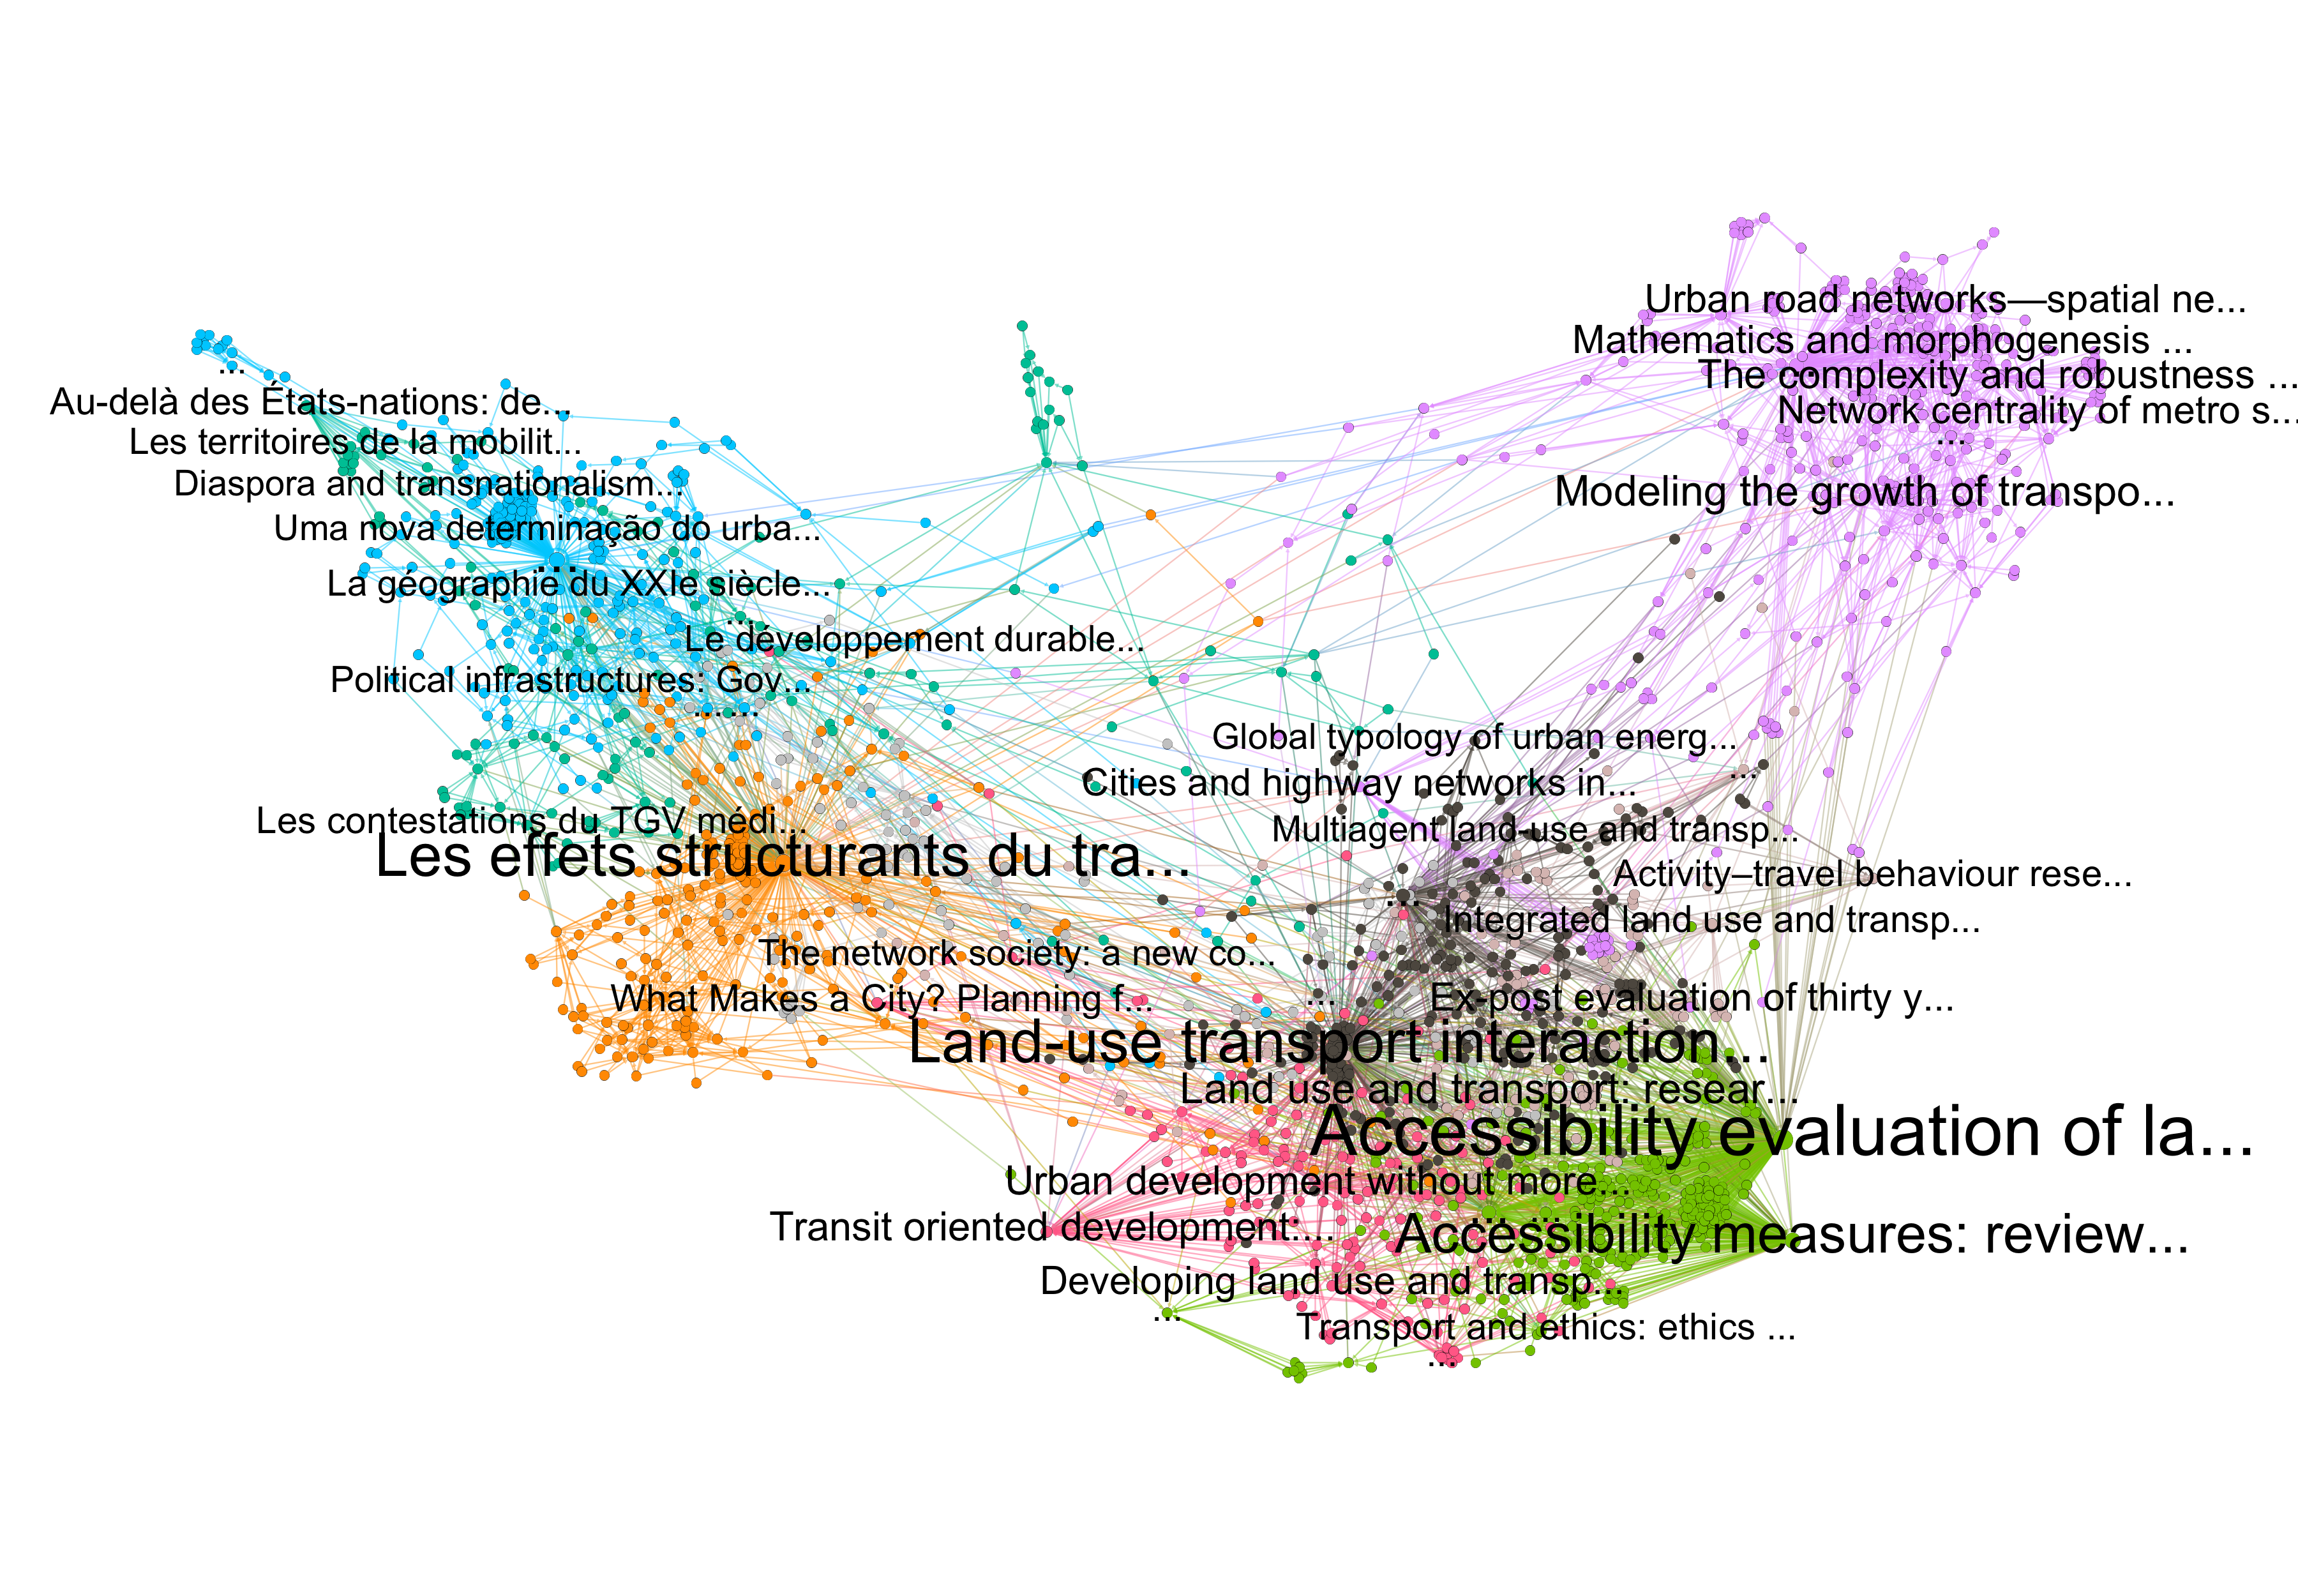
\includegraphics[width=\linewidth]{Figures/QuantEpistemo/rawcore_labs36.png}
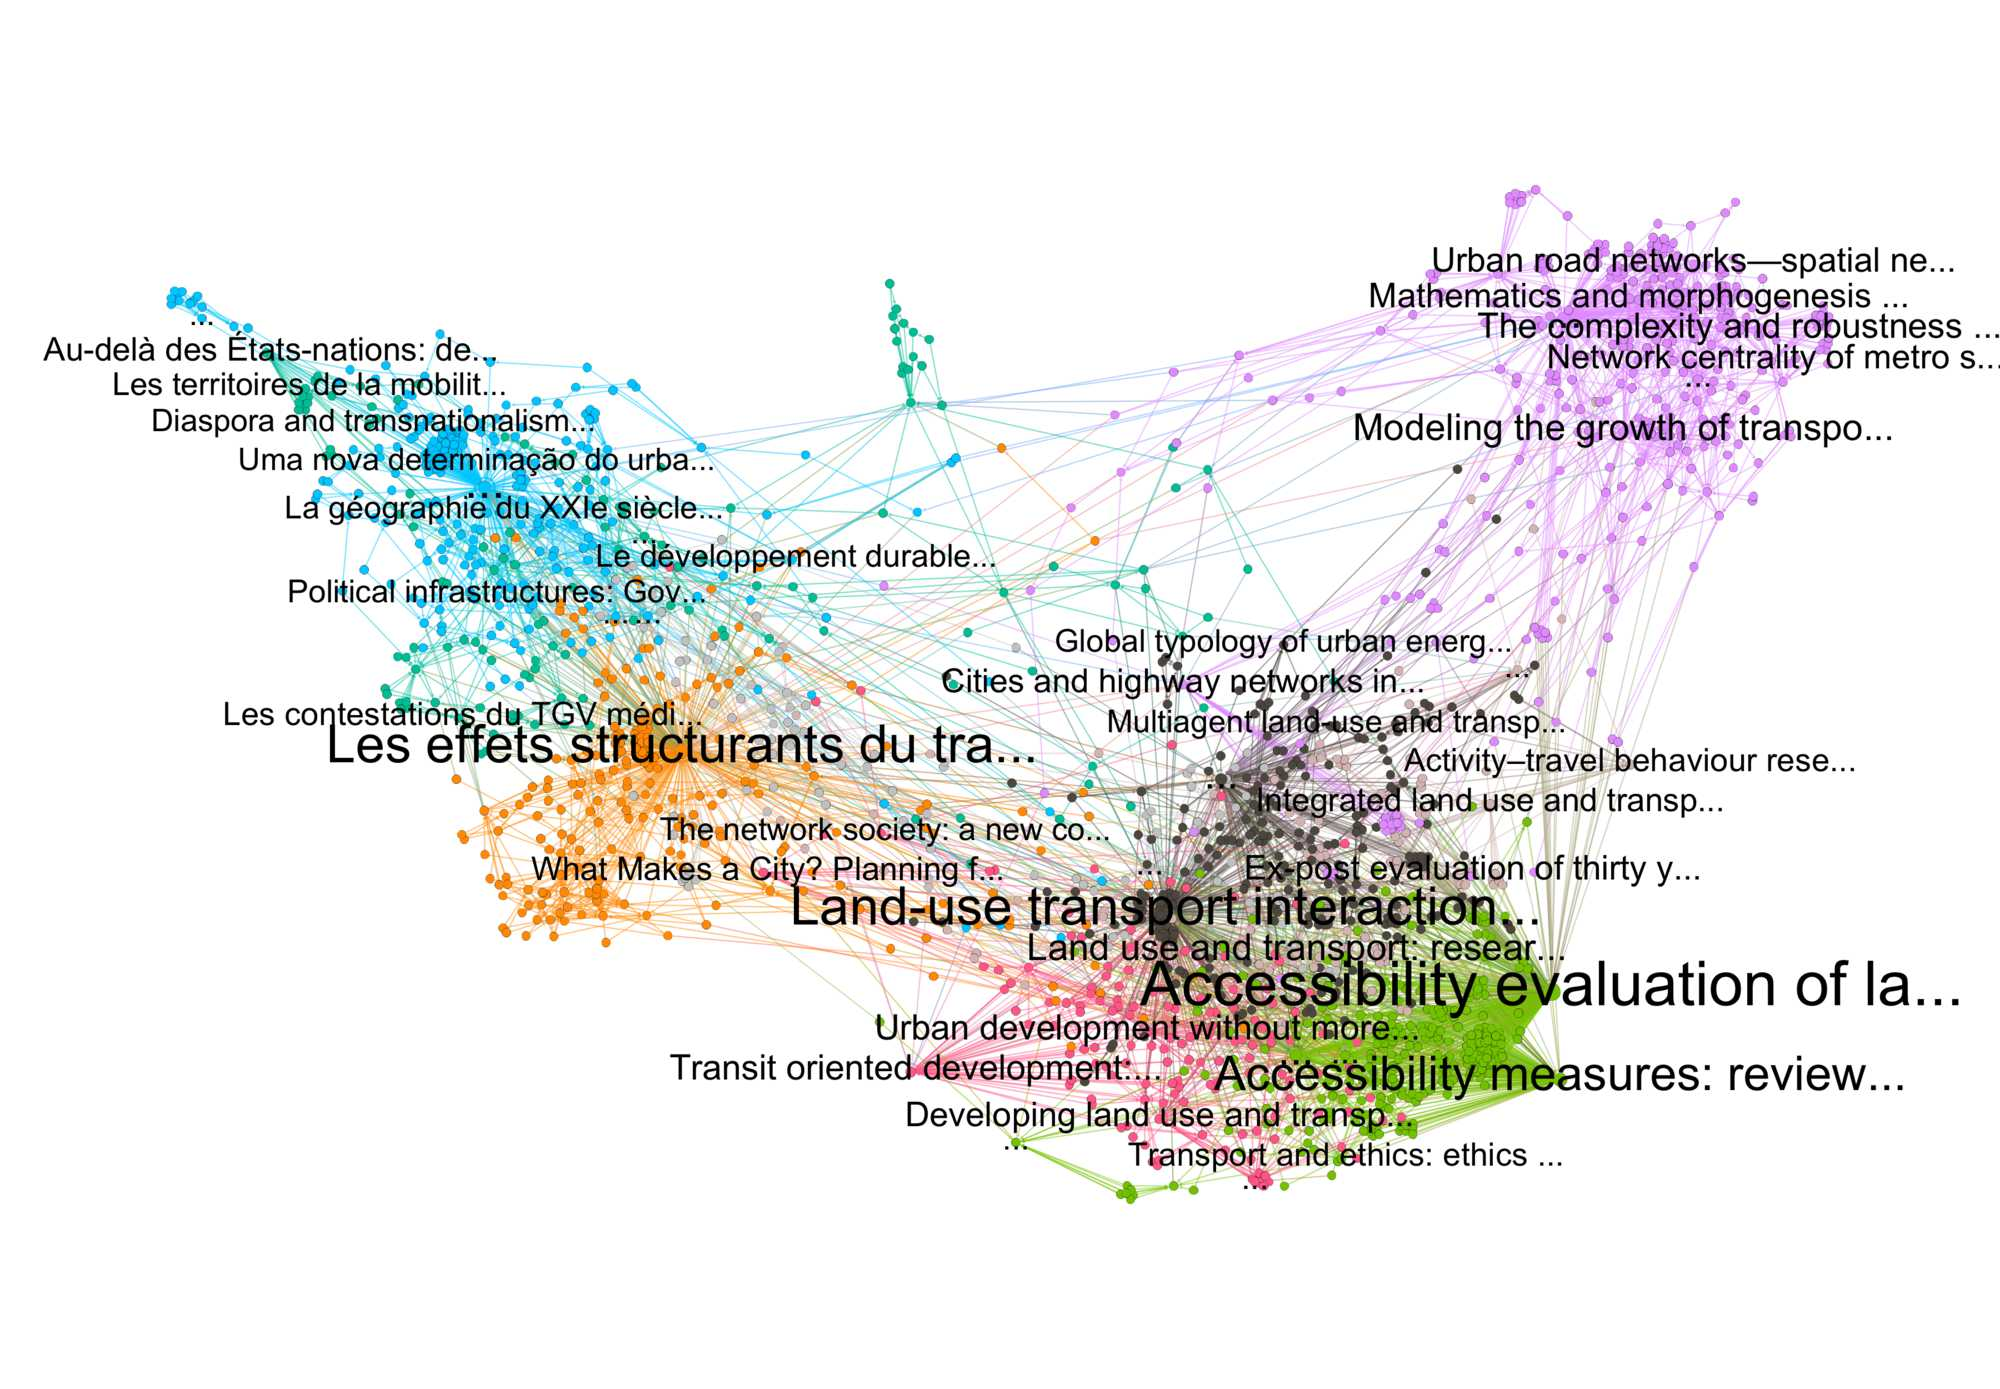
\includegraphics[width=\linewidth]{figures/2-2-2-fig-quantepistemo-citnw.jpg}
\caption[Citation Network][Réseau de citations]{\textbf{Citation Network.} We visualize references having at least two links, using a force-atlas algorithm. Colors give communities described in text. In orange, blue, turquoise: urban geography, transport geography, political sciences; in pink, black, green: planning, accessibility, LUTI; in purple: spatial networks (physics and economics).\label{fig:quantepistemo:citnw}}
\end{figure}
%%%%%%%%%%%%%%%%%

\paragraph{Semantic communities}


The extraction of keywords is done following an heuristic inspired by~\cite{chavalarias2013phylomemetic}. The complete description of the method and its implementation if given in Appendix~\ref{app:sec:cybergeo}. It is based on second-order relations between semantic entities, which are \emph{n-grams}, i.e. multiple keywords which can have a length up to three. These are estimated by the intermediate of the co-occurence matrix, which statistical properties yield a measure of deviation from uniform co-occurrences, which is used to evaluate the relevance of keywords. By selecting a fixed number of relevant keywords $K_W = 10000$, we can then construct a network weighted by co-occurrences.

The topology of the raw network does not allow the extraction of clear communities, in particular because of the presence of hubs that correspond to frequent terms common to many fields (e.g. \texttt{model}, \texttt{space}). These words are used in a comparable way in all the studied fields, and do not carry information to separate them\footnote{But they will carry some if we were comparing a corpus in quantitative geography and a corpus in musicology for example.}. We make the assumption that these highest degree terms do not carry specific information on particular classes and can be thus filtered given a maximal degree threshold $k_{max}$ (we are thus interested in what makes the specificity of each domain). Similarly, edges with small weight are considered as noise and filtered according to a minimal edge weight threshold $\theta_w$. The generic method furthermore allows a preliminary filtration of keywords, according to a document frequency window $\left[ f_{min},f_{max} \right]$, to which results are not sensitive in our case. The sensitivity analysis of the characteristics of the filtered network, in particular its size, modularity and community structure, is given in Fig.~\ref{fig:sensitivity}. We choose parameter values allowing a multi-objective optimization between modularity and network size, $\theta_w = 10,k_{max} = 500$, by the choice of a compromise point on a Pareto front, what gives a semantic network of size $(V=7063,E=48952)$. It is visualized in Appendix~\ref{app:sec:quantepistemo}.

We then retrieve communities in the network using a standard Louvain clustering on the optimal filtered network. We obtain 20 communities for a modularity of 0.58. These are examined manually to be named, the automatic naming techniques~\cite{yang2000improving} being not elaborated enough to make the implicit distinction between thematic and methodological fields for example (in fact between knowledge domains, see~\ref{sec:knowledgeframework}) which is a supplementary dimension that we do not tackle here, but necessary to have meaningful descriptions. The communities are described in Table~\ref{tab:quantepistemo:semanticdomains}. We directly see the complementarity with the citation approach, since emerge here together subjects of study (High Speed Rail, Maritime Networks), domains and methods (Networks, Remote Sensing, Mobility Data Mining), thematic domains (Policy), pure methods (Agent-based Modeling, Measuring). Thus, a reference may use several of these communities. We furthermore have a finer granularity of information. The effect of language is strong since French geography is distinguished as a separated category (advanced analyses could be considered to better understand this phenomenon and benefit from it: sub-communities, reconstruction of a specific network, studies by translation; but these are out of purpose in this exploratory study). We note the importance of networks, and of problematics in political sciences and socio-economic. We will use the first category in most models we will develop, but keeping in mind the importance of problematics linked to governance, we will proceed to a specific study in~\ref{sec:lutecia}.



%%%%%%%%%%%%%%
\begin{table}
\caption[Semantic communities][Communautés sémantiques]{\textbf{Description of semantic communities.} We give their size, their proportion in quantity of keywords (under the form of \emph{multi-stems}) cumulated on the full corpus, and representative keywords selected by maximal degree.\label{tab:quantepistemo:semanticdomains}}
\begin{tabular}{llll}
\hline\noalign{\smallskip}
Name & Size & Weight & Keywords  \\
\noalign{\smallskip}\hline\noalign{\smallskip}
Networks & 820 & 13.57\% & \texttt{social network, spatial network, resili} \\
Policy & 700 & 11.8\% & \texttt{actor, decision-mak, societi} \\
Socio-economic & 793 & 11.6\% & \texttt{neighborhood, incom, live} \\
High Speed Rail & 476 & 7.14\% & \texttt{high-spe, corridor, hsr} \\
French Geography & 210 & 6.08\% & \texttt{système, développement, territoire} \\
Education & 374 & 5.43\% & \texttt{school, student, collabor} \\
Climate Change & 411 & 5.42\% & \texttt{mitig, carbon, consumpt} \\
Remote Sensing & 405 & 4.65\% & \texttt{classif, detect, cover} \\
Sustainable Transport & 370 & 4.38\% & \texttt{sustain urban, travel demand, activity-bas} \\
Traffic & 368 & 4.23\% & \texttt{traffic congest, cbd, capit} \\
Maritime Networks & 402 & 4.2\% & \texttt{govern model, seaport, port author} \\
Environment & 289 & 3.79\% & \texttt{ecosystem servic, regul, settlement} \\
Accessibility & 260 & 3.23\% & \texttt{access measur, transport access, urban growth} \\
Agent-based Modeling & 192 & 3.18\% & \texttt{agent-bas, spread, heterogen} \\
Transportation planning & 192 & 3.18\% & \texttt{transport project, option, cba} \\
Mobility Data Mining & 168 & 2.49\% & \texttt{human mobil, movement, mobil phone} \\
Health Geography & 196 & 2.49\% & \texttt{healthcar, inequ, exclus} \\
Freight and Logistics & 239 & 2.06\% & \texttt{freight transport, citi logist, modal} \\
Spanish Geography & 106 & 1.26\% & \texttt{movilidad urbana, criteria, para} \\
Measuring & 166 & 1.0\% & \texttt{score, sampl, metric} \\
\noalign{\smallskip}\hline
\end{tabular}
\end{table}
%%%%%%%%%%%%%

\paragraph{Measures of interdisciplinarity}

Distribution of keywords within communities provides an article-level interdisciplinarity. The combination of citation and semantic layers in the hyper-network provide second-order interdisciplinarity measures (semantic patterns of citing or cited), that we don't use here because of the modest size of the citation network (see \ref{app:sec:cybergeo} and \ref{app:sec:patentsmining}). More precisely, a reference $i$ can be viewed as a probability vector on semantic classes $j$, that we write in a matrix form $\mathbf{P}=(p_{ij})$. These are simply estimated by the proportions of keywords classified in each class for the reference. A classical measure of interdiscplinarity~\cite{bergeaud2017classifying} is then $I_i = 1 - \sum_j p_{ij}^2$. Let $\mathbf{A}$ be the adjacency matrix of the citation network, and let $\mathbf{I}_k$ matrices selecting rows corresponding to class $k$ of the citation classification: $Id\cdot \mathbbm{1}_{c(i)=k}$, such that $I_k \cdot A \cdot I_{k'}$ gives exactly the citations from $k$ to $k'$. The citation proximity between citation communities is then defined by $c_{kk'} = \sum \mathbf{I}_k \cdot \mathbf{A} \cdot \mathbf{I}_{k'} /  \sum \mathbf{I}_k \cdot \mathbf{A}$. We define the semantic proximity by defining a distance matrix between references by $\mathbf{D} = d_{ii'}=\sqrt{\frac{1}{2}\sum (p_{ij}-p{i'j})^2}$ and the semantic proximity by $s_{kk'} = \mathbf{I}_k \cdot \mathbf{D} \cdot \mathbf{I}_{k'} / \sum \mathbf{I}_k \sum \mathbf{I}_{k'}$.


We show in Fig.~\ref{fig:quantepistemo:interdisc} the values of these different measures, and also the semantic composition of citation communities, for the main semantic classes. The distribution of $I_i$ shows that articles orbiting in the LUTI field are the most interdisciplinary in the terms used, what could be due to their applied character. Other disciplines show similar patterns, except geography and infrastructure planning which exhibit quasi-uniform distributions, witnessing the existence of very specialized references in these classes. This is not necessarily stunning, given the targeted sub-fields exhibited (political sciences for example, and similarly prospective studies of type cost-benefit are very narrow). This first crossing of the layers confirms the specificities of each field. Regarding semantic compositions, most act as an external validation given the dominant classes. The field which is the less concerned by socio-economical issues is infrastructure planning, what could give reason to critics of technocracy. Issues on climate change and sustainability are relatively well dispatched. Finally, geographical works are mostly related to governance issues.

Proximity matrices confirm the conclusion obtained previously in terms of citation, the sharing being very low, the highest values being up to one fourth of planning towards geography and of LUTI towards TOD (but not the contrary, the relations can be in a unique sense). But semantic proximities show for example that LUTI, TOD, Accessibility and Networks are close in their terms, what is logical for the first three, and confirms for the last that physicists mainly rely on methods of this fields linked to planning to legitimate their works. Geography is totally isolated, its closest neighbor being infrastructure planning. This study is very useful in our context, since it shows compartmentalized domains sharing terms, and thus a priori some common problematics and subjects. Domains do not speak to each other while speaking languages that are not that far, hence the increased relevance to aim at harmonizing their music in our work: our models will have to use elements, ontologies and scales of these different fields.


%%%%%%%%%%%%%%%%%%
\begin{figure}
%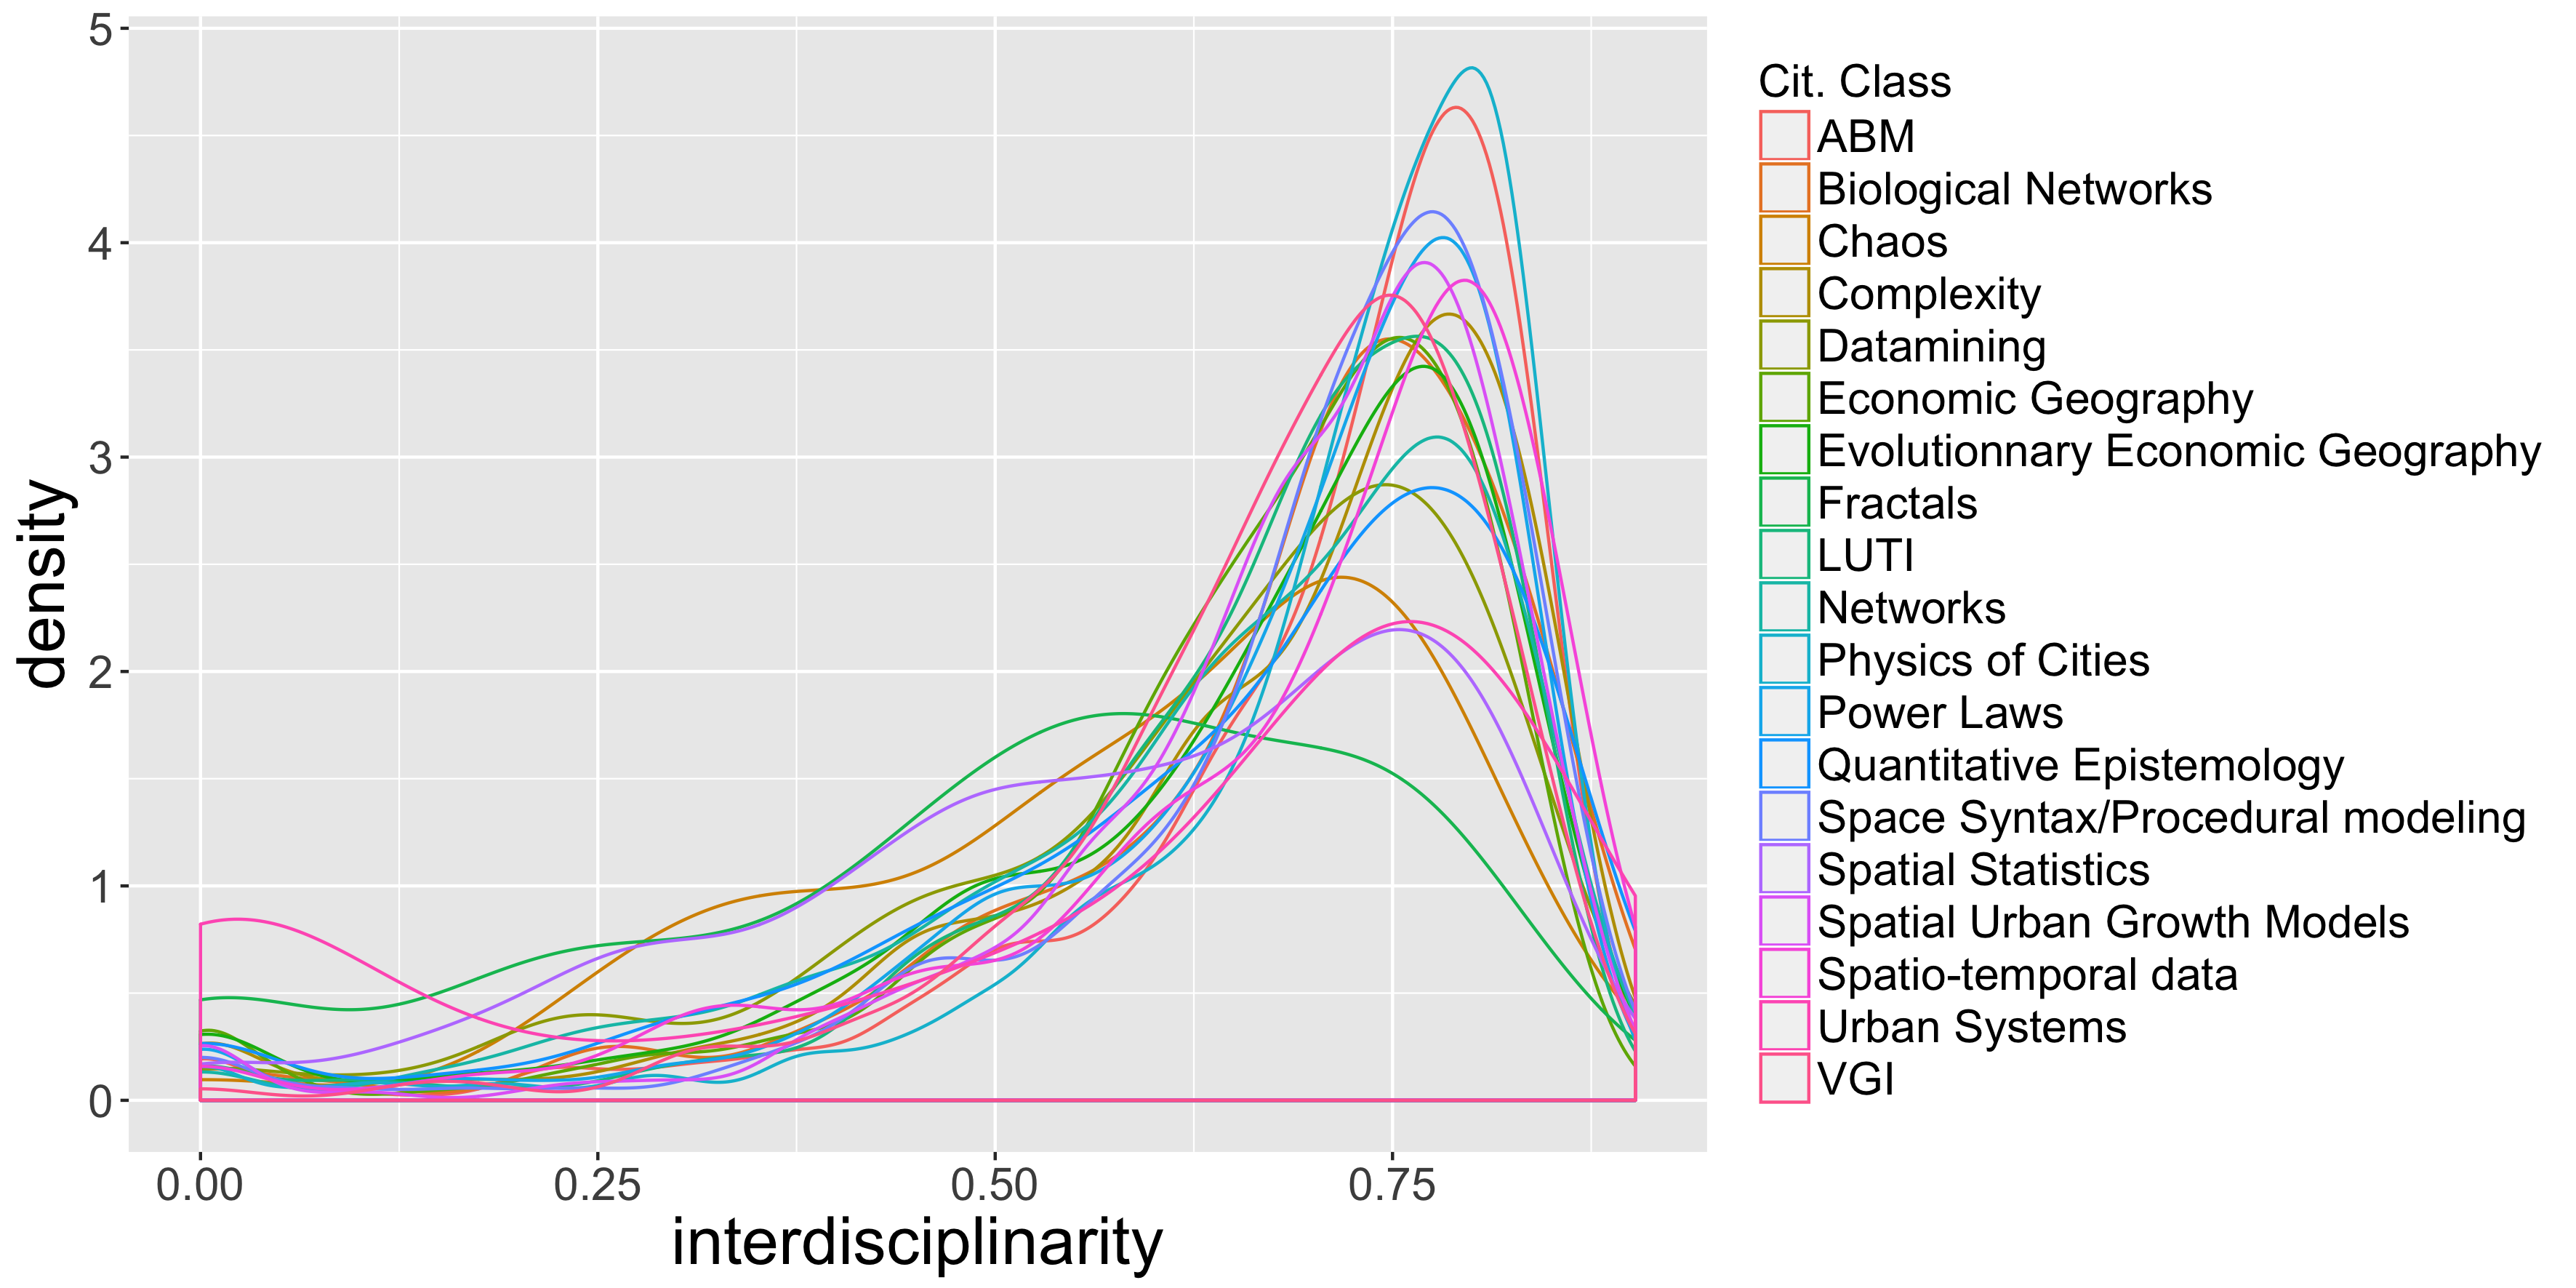
\includegraphics[width=0.49\linewidth]{Figures/QuantEpistemo/interdisciplinarities}
%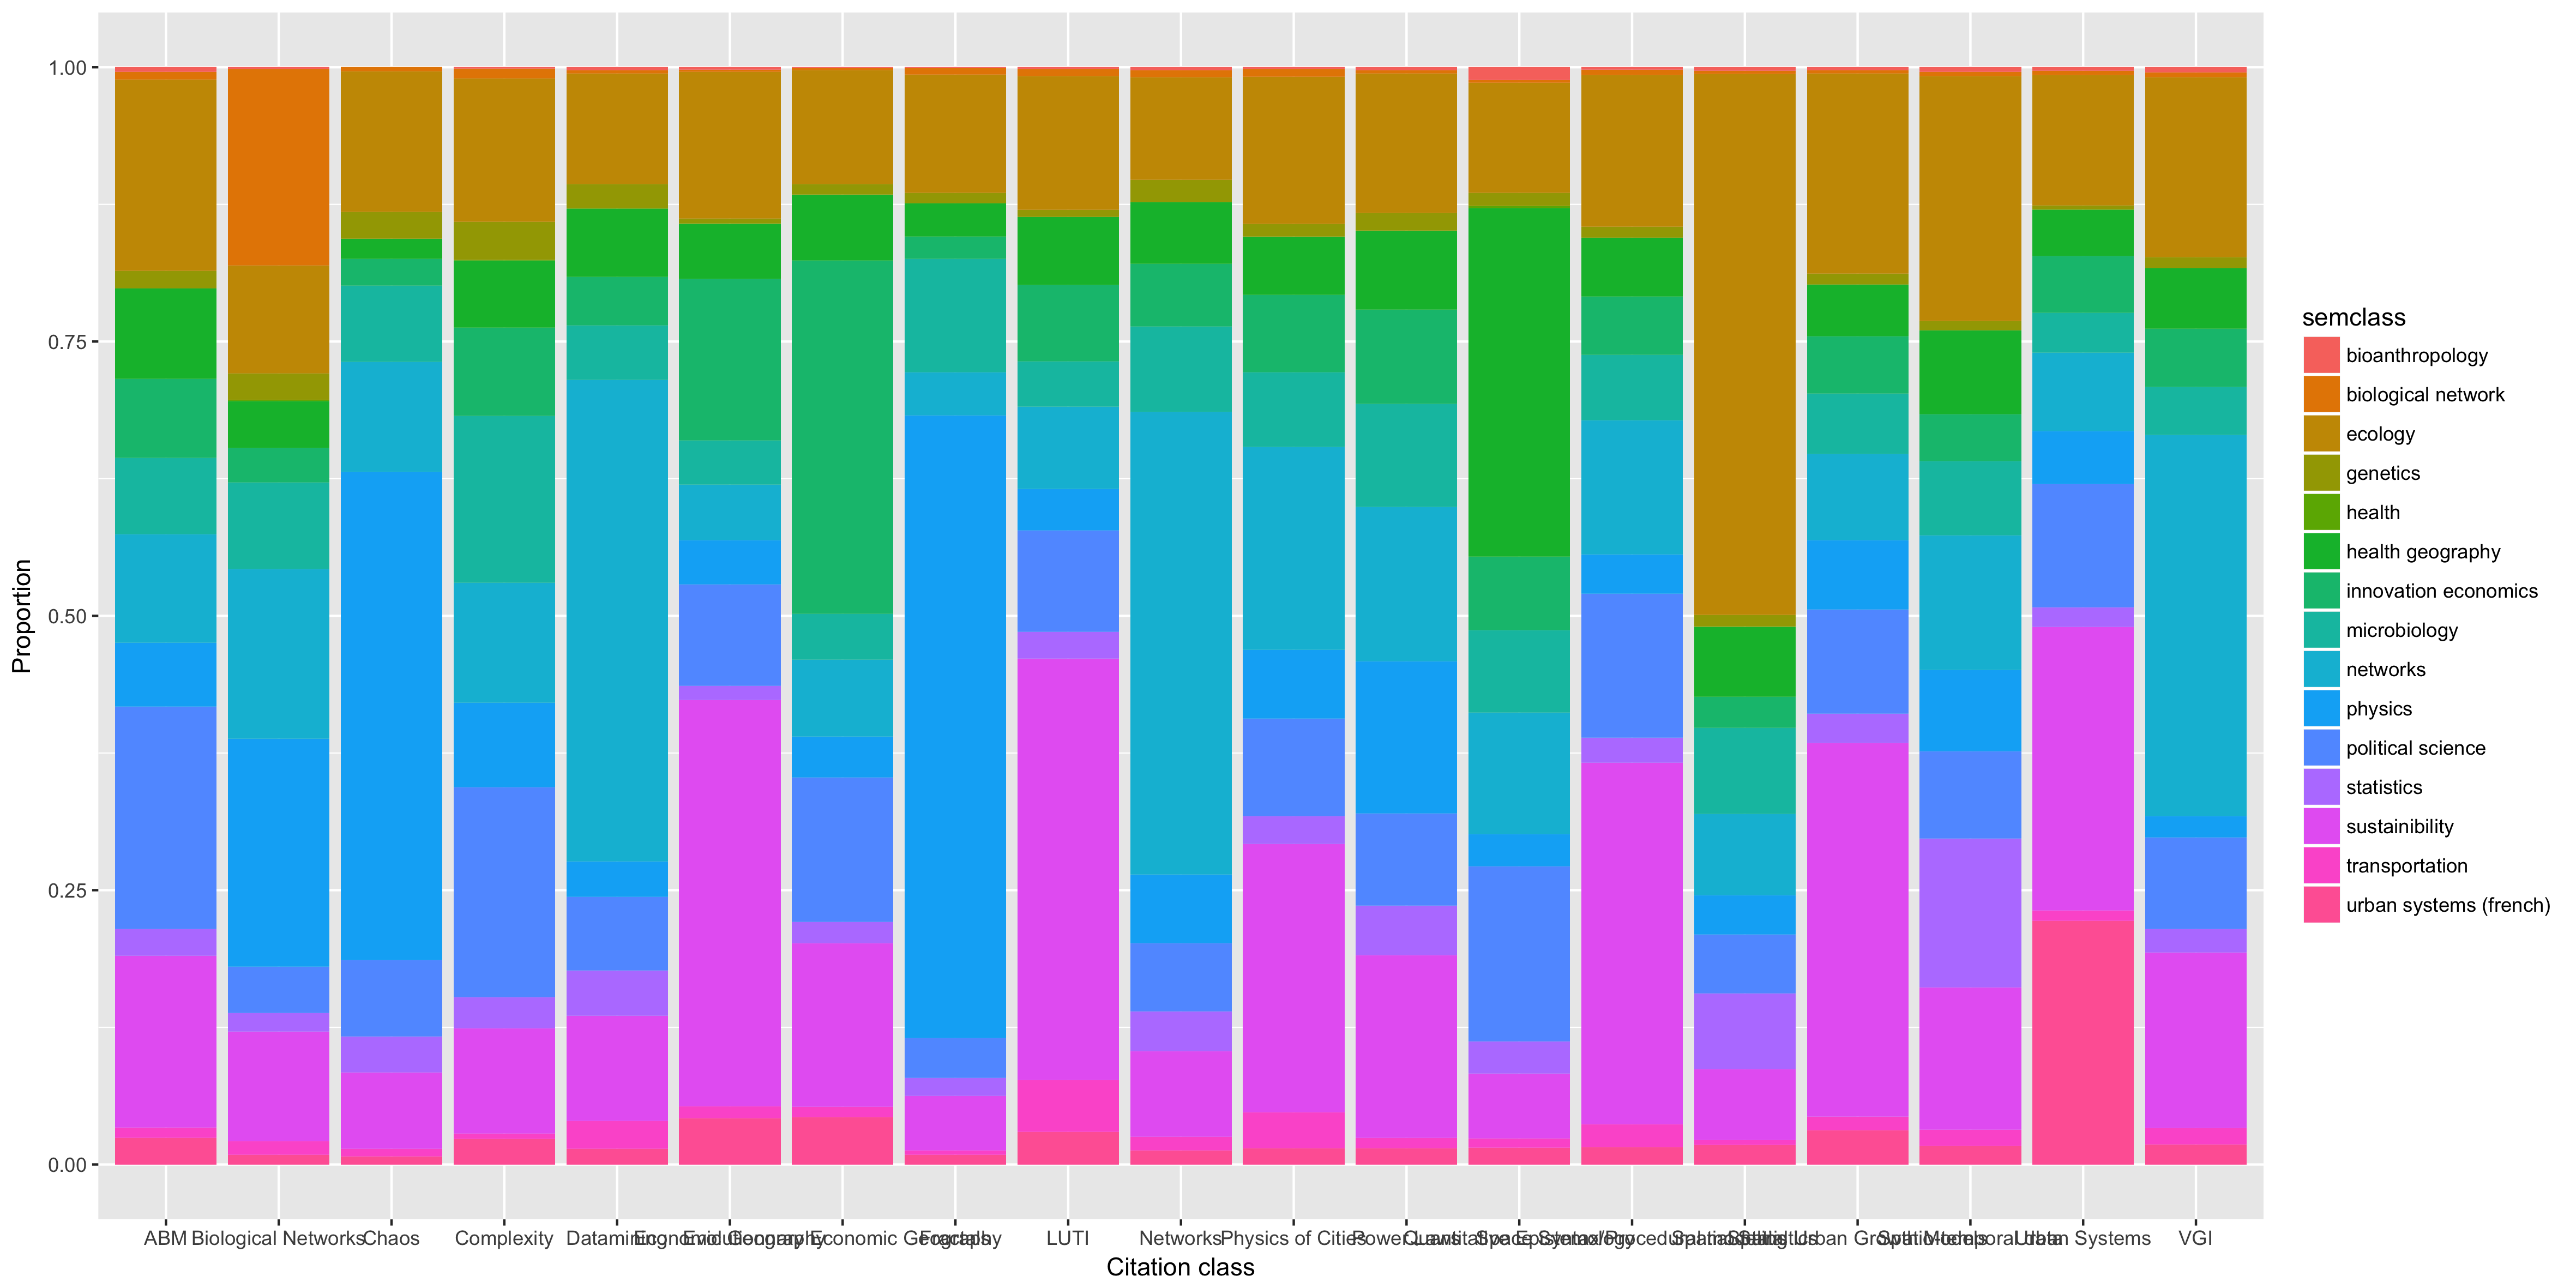
\includegraphics[width=0.49\linewidth]{Figures/QuantEpistemo/compo_proportion}\\
%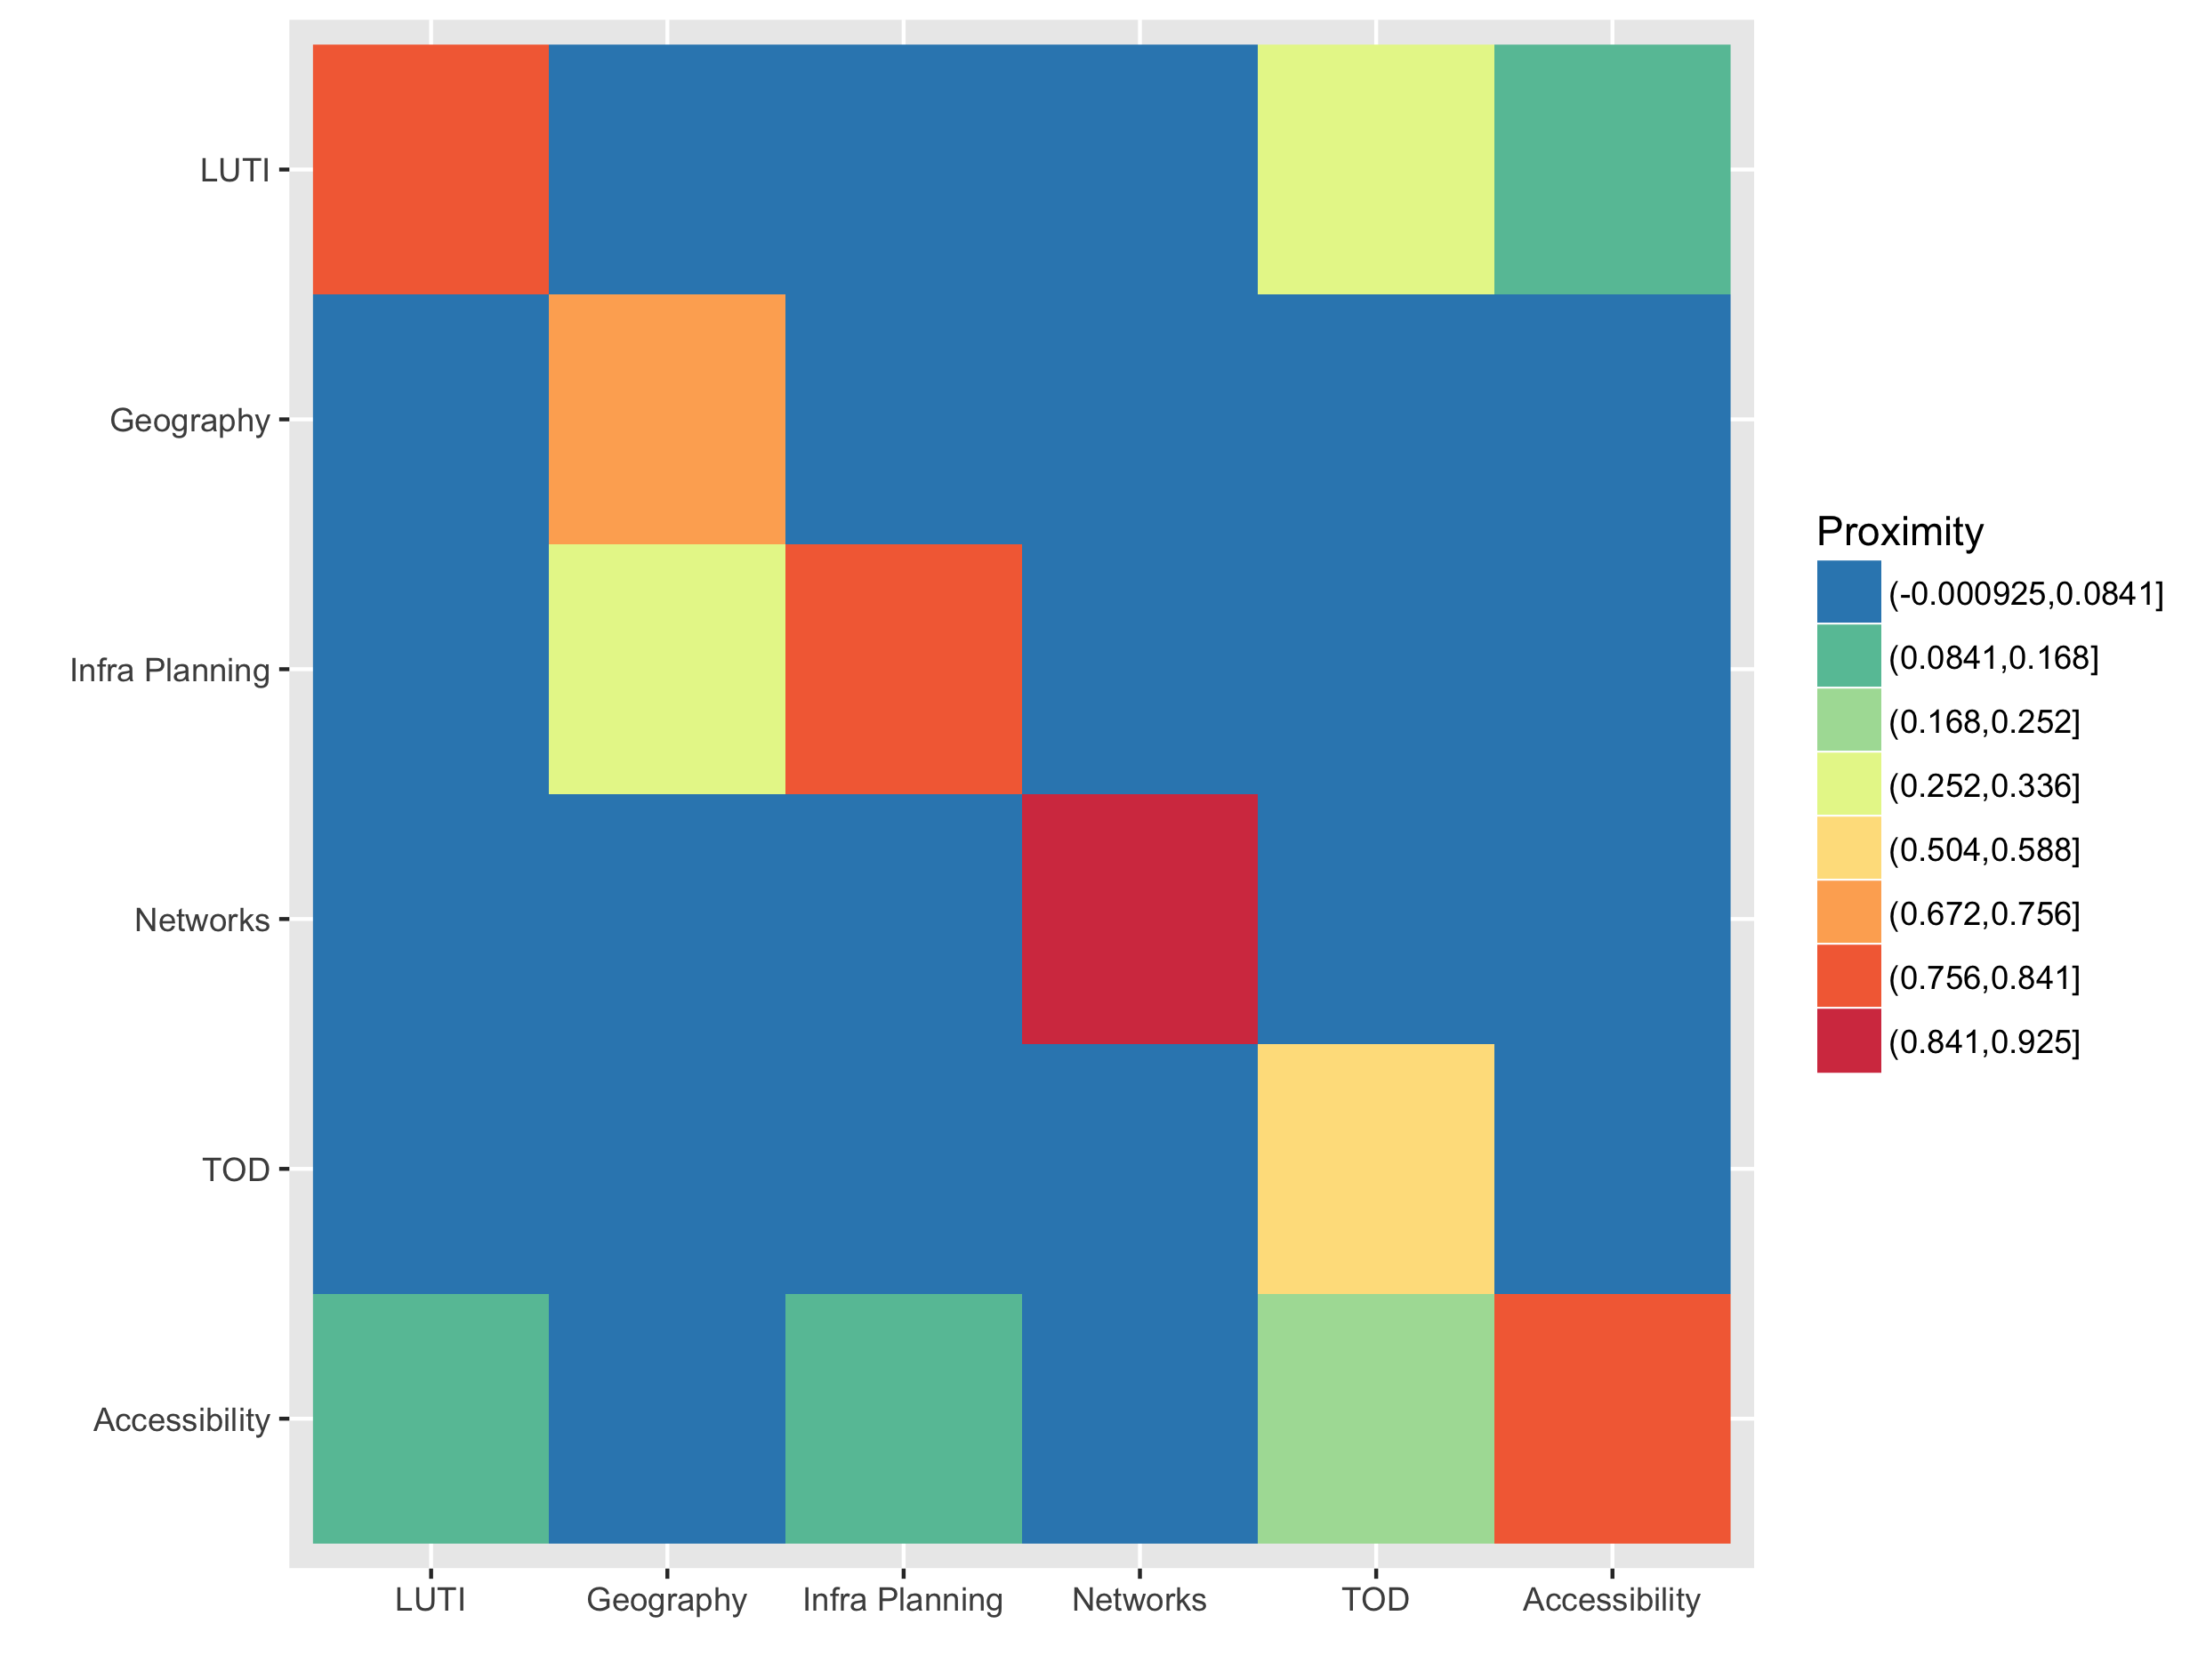
\includegraphics[width=0.49\linewidth]{Figures/QuantEpistemo/citation_proximities}
%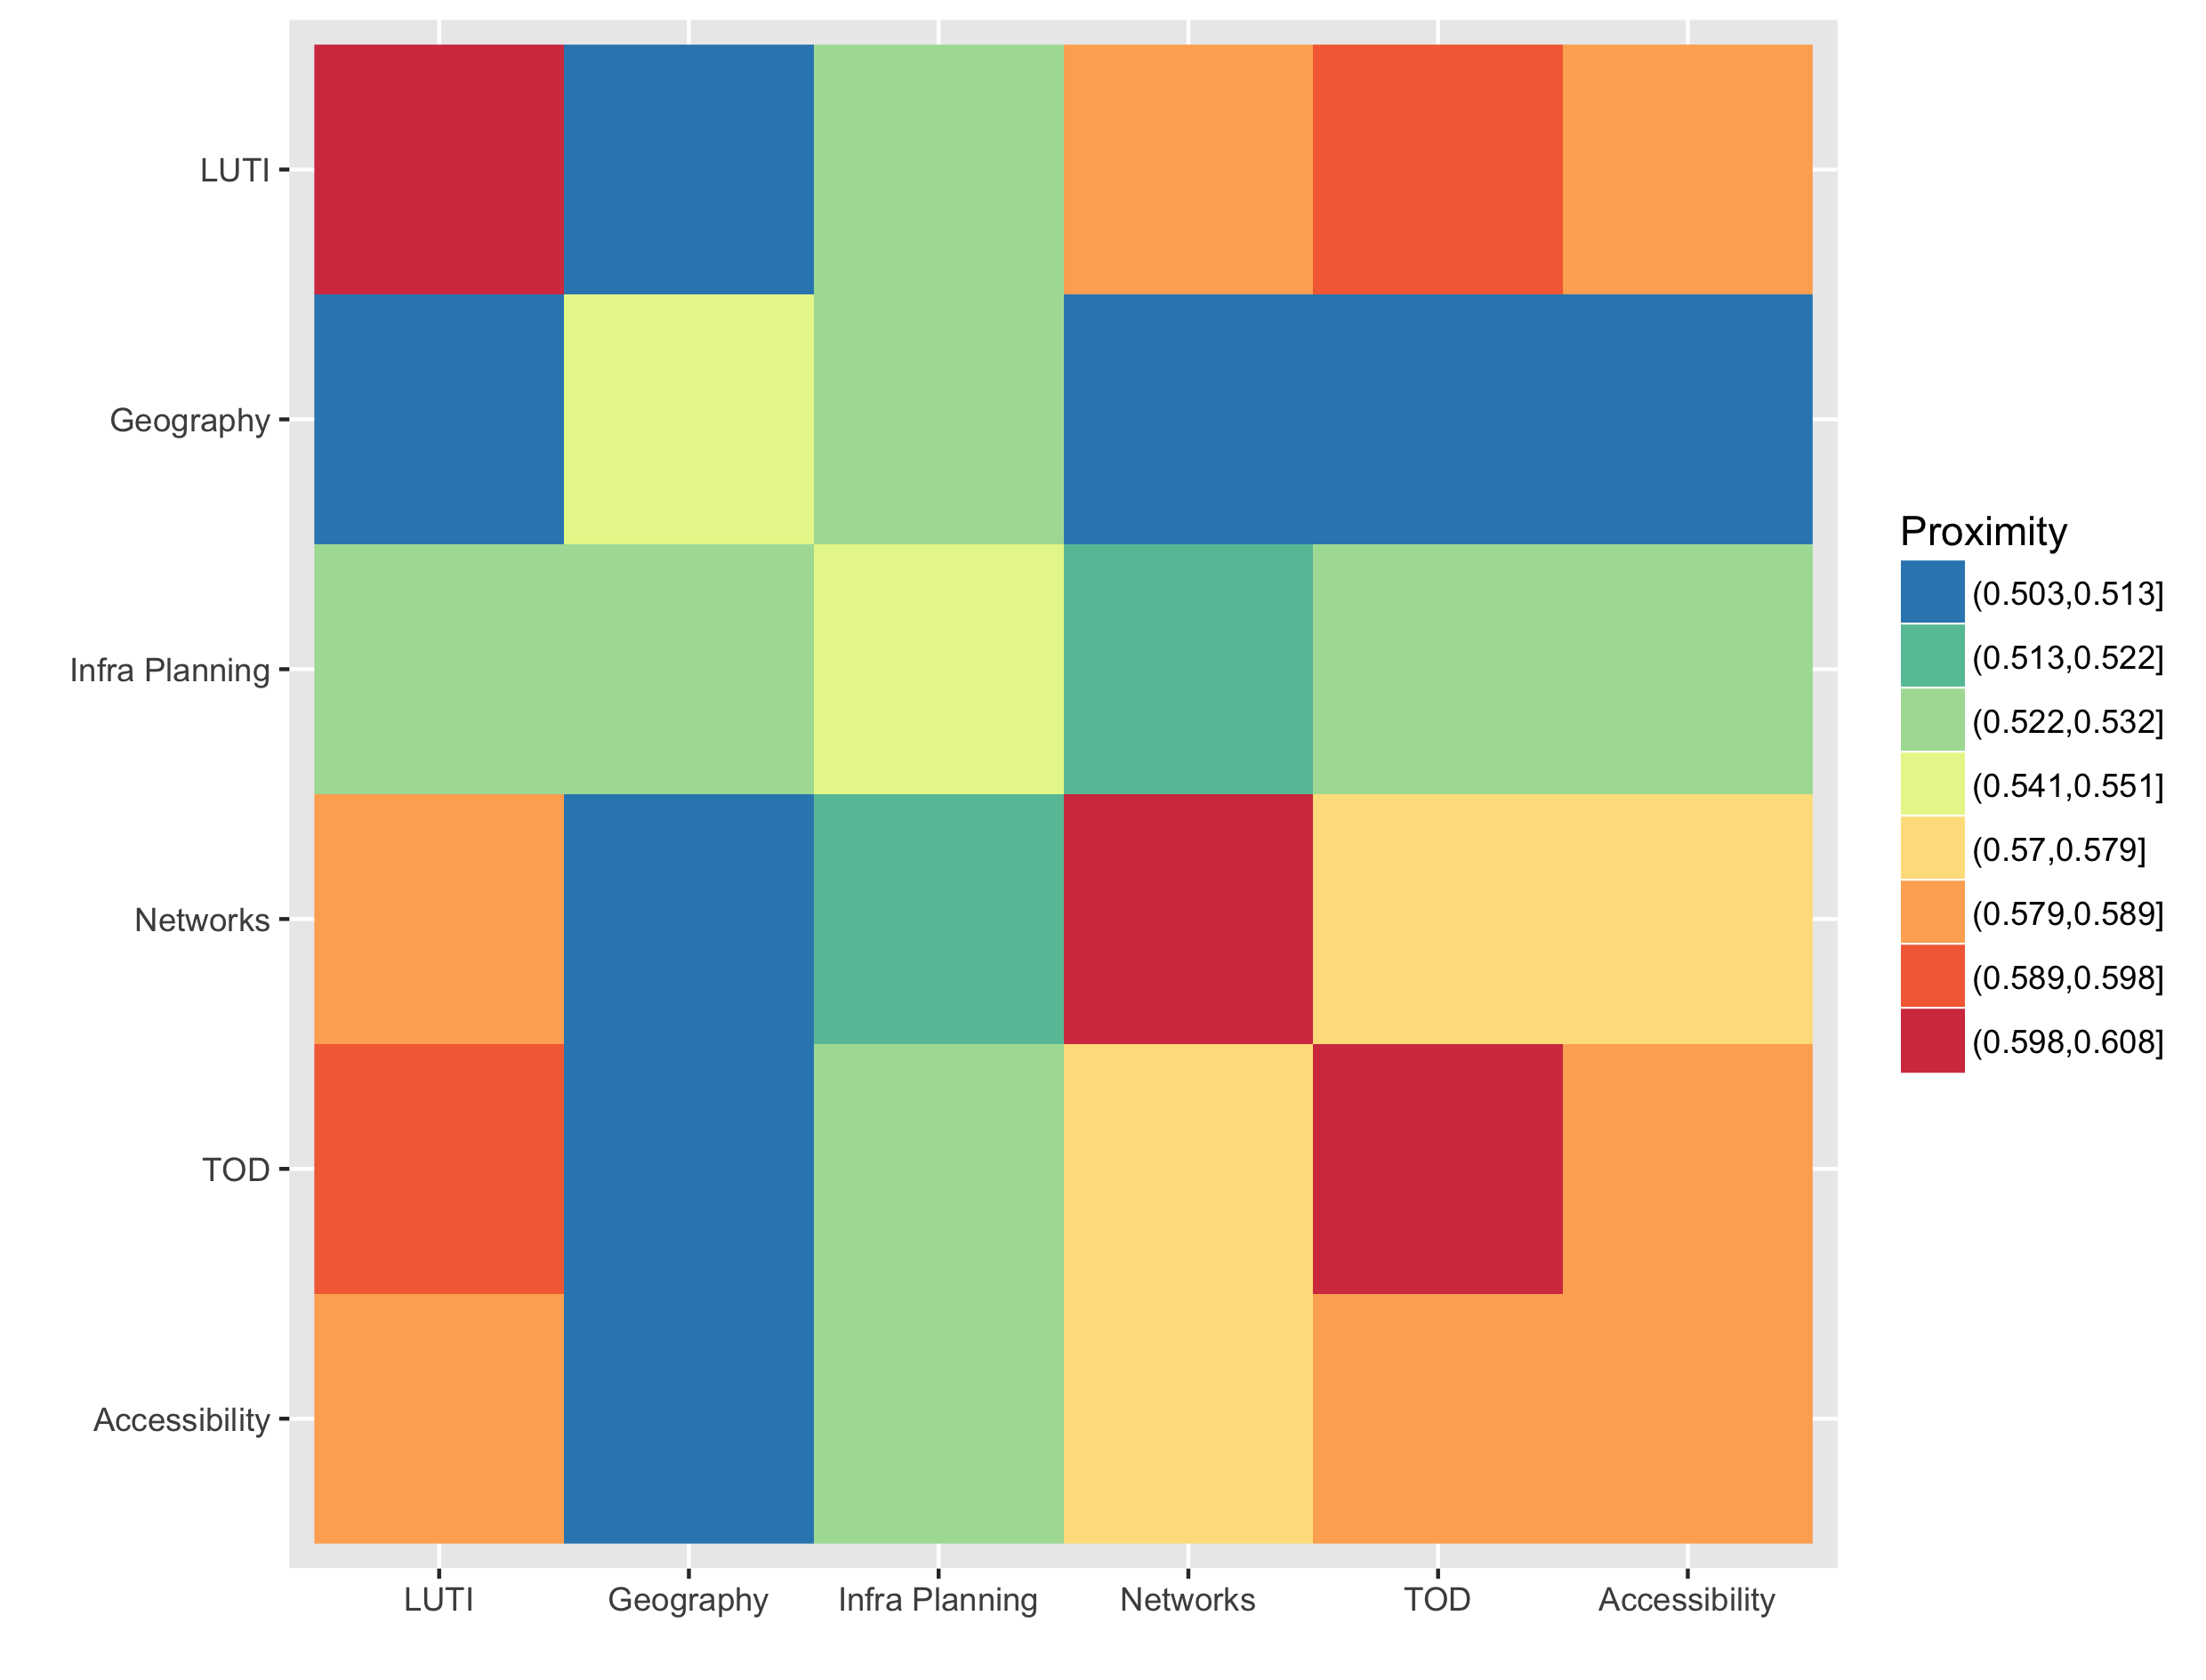
\includegraphics[width=0.49\linewidth]{Figures/QuantEpistemo/semantic_proximities}
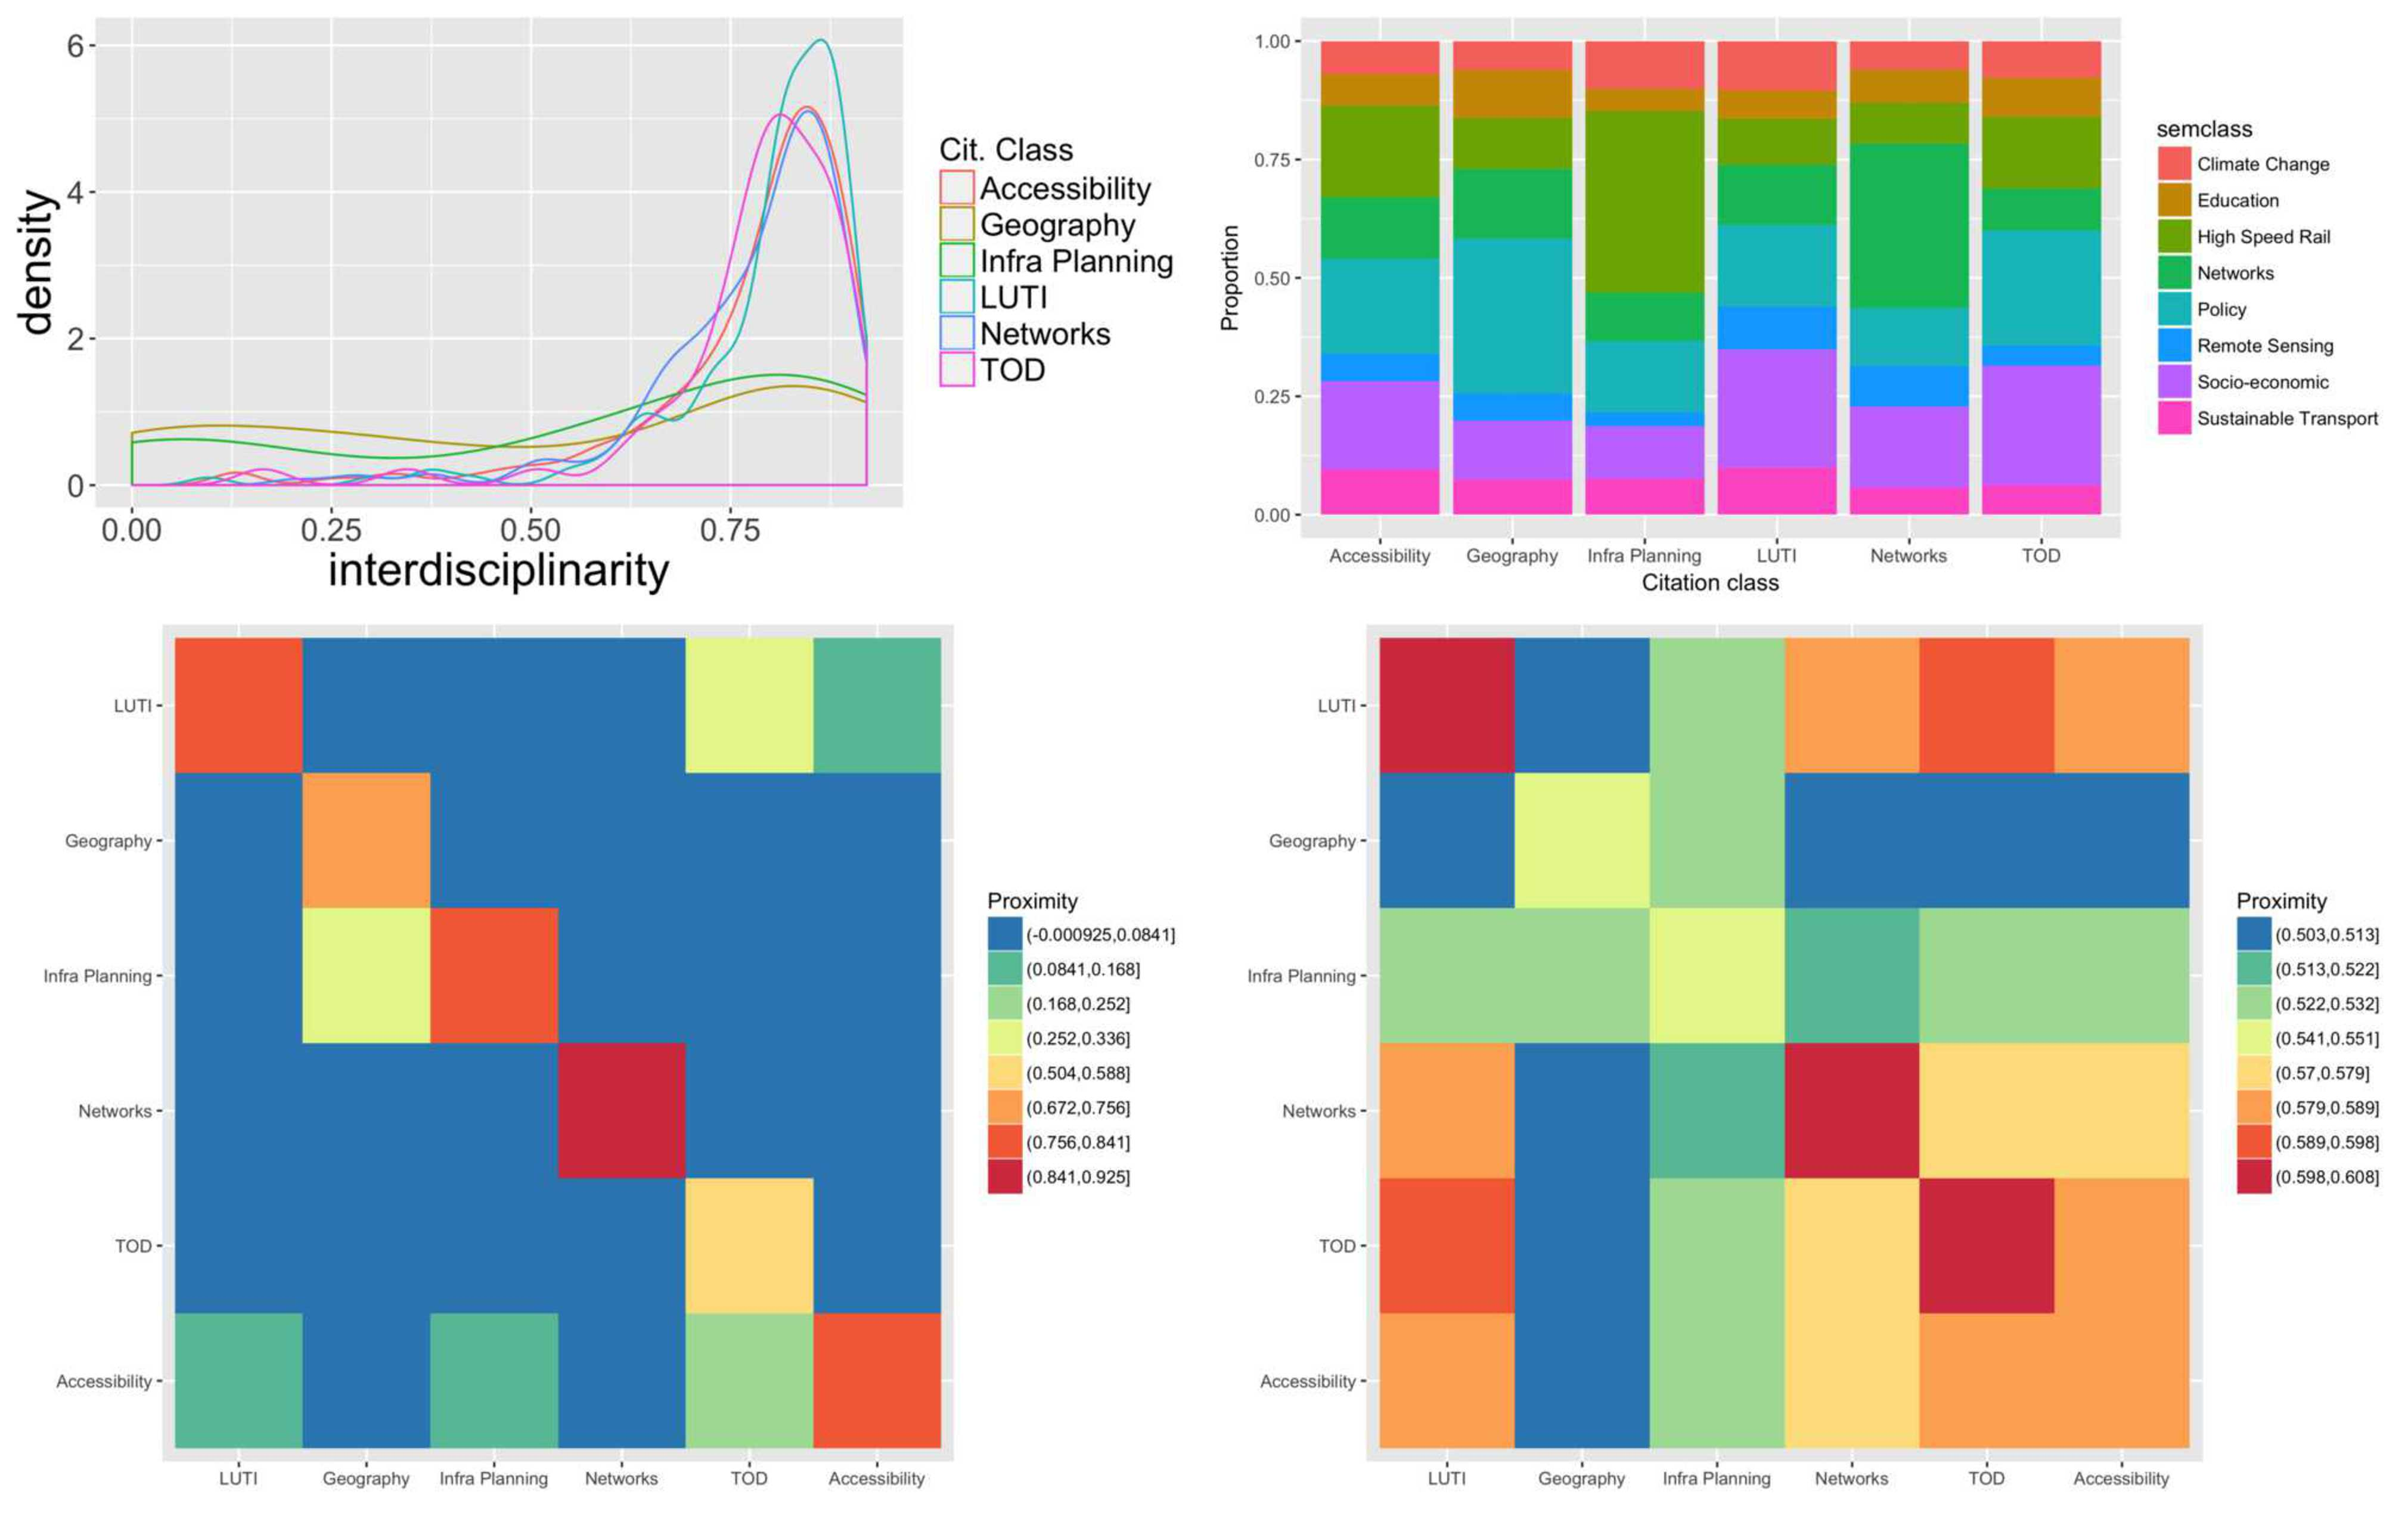
\includegraphics[width=\linewidth]{Figures/Final/2-2-2-fig-quantepistemo-interdisc.jpg}
\caption[Patterns of interdisciplinarity][Motifs d'interdisciplinarité]{\textbf{Patterns of interdisciplinarity.} \textit{(Top Left)} Statistical distribution of $I_i$ by citation classes, in other words distribution of interdisciplinarity levels within citation classes; \textit{(Top Right)} Semantic composition of citation classes: for each citation class (in abscissa), the proportion of each semantic class (in color) is given; \textit{(Bottom Left)} Citation proximity matrix for $c_{kk'}$ between citation classes; \textit{(Bottom Right)} Semantic proximity matrix $s_{kk'}$ between citation classes. \label{fig:quantepistemo:interdisc}}
\end{figure}
%%%%%%%%%%%%%%%%%%


We conclude this analysis with a more robust approach to quantify proximities between the layers of the hypernetwork. It is straightforward to construct a correlation matrix between two classifications, through the correlations of their columns. We define the probabilities $\mathbf{P}_C$ all equal to 1 for the citation classification. The correlation matrix between it and $\mathbf{P}$ extends from -0.17 to 0.54 and has an average with an absolute value of 0.08, what is significant in comparison to random classifications since a bootstrap with $b=100$ repetitions with shuffled matrices gives a minimum at $-0.08 \pm 0.012$, a maximum at $0.11 \pm 0.02$ and an absolute average at $0.03 \pm 0.002$. This shows that the classifications are complementary and that this complementarity is statistically significant compared to random classifications. The adequacy of the semantic classification in relation to the citation network can also be quantified by the multi-classes modularity~\cite{nicosia2009extending} (see~\ref{app:sec:patentsmining} for a mathematical definition), which translates the likelihood that a link is due to the classification studied, taking into account the simultaneous belonging to multiple classes. Thus, the multi-class modularity of semantic probabilities for the citation network s 0.10, what on one side is a significant sign of an adequacy, a bootstrap still with $b=100$ giving a value of $0.073 \pm 0.003$, which remains limited given the maximal value fixed by citation probabilities within their own network which give a value of 0.81, what conform furthermore the complementarity of classifications.







%%%%%%%%%%%%%%%
\section{Discussion}
%%%%%%%%%%%%%%%


We have thus in this section sketched an overview of disciplines in relation with our subject, and also their relations. We will aim in the next section at understanding with more details their ``content'', i.e. the means used to solve the problems encountered.

We briefly give directions to extend the analysis we just did and also implications for the epistemological positioning of our work.

A possible direction to strengthen our quantitative epistemological analysis would be to work on full textes related to the modeling of interaction between networks and territories, with the aim to automatically extract thematics within articles. Methods more suited for full texts than the one used here for example include Latent Dirichlet Allocation~\cite{blei2003latent}. The idea would be to perform some kind of automatized modelography, extending the modelography methodology developed by~\cite{schmitt2013modelographie}, to extract characteristics such as ontologies, model architecture or structures, scales, or even typical parameter values. It is not clear to what extent the structure of models can be extracted from their description in papers and it surely depends on the discipline considered. For example in a framed field such as transportation planning, using a pre-defined ontology (in the sense of dictionary) and a fuzzy grammar could be efficient to extract information as the discipline has relatively strict conventions. In theoretical and quantitative geography, beyond the barrier of diversity of possible formalizations for a same ontology, the organisation of information is surely more difficult to grasp through unsupervised data-mining because of the more literary nature of the discipline: synonyms and figures of speech are generally the norm in good level human sciences writing, fuzzing a possible generic structure of knowledge description.

The methodology developed here is efficient to offer reflexivity instruments, i.e. it can be used to study our approach itself. One of its application, beyond the one on the scientific journal Cybergeo in a perspective of Open Science (see Appendix~\ref{app:sec:cybergeo}), will be to our own corpus of references, with the aim to reveal possible research directions or exotic issues. It is eventually possible to do it in a dynamical way, thanks to the \texttt{git} history which allows to recover any version of the bibliography at a given date on the three years elapsed. The aim will also be to understand our knowledge production patterns in order to contribute to~\ref{sec:knowledgeframework}. The detailed development is done in Appendix~\ref{app:reflexivity}.







%%%%%%%%%%%%%%%
\section{Conclusion}
%%%%%%%%%%%%%%%


This section thus allowed us to sketch a landscape of disciplines in relation with our problematic, and of relations between these disciplines, in terms of citations but also of level of interdisciplinarity.







%%%%%%%
%% Biblio
%%%%%%%


\bibliographystyle{jtlu}
\bibliography{biblio}




\end{document}


%%%%%%%%%%%
%% Template
%%%%%%%%%%%




%%%%%%%%%%
%\begin{figure*}[htbp]
%  \centering
%  \includegraphics{fig1}
%  \caption{Caption ...  }
%  \label{fig:1}
%\end{figure*}




